%\documentclass[10pt,preprint]{aastex}  % for e-submission to ApJ
%\documentclass[12pt,preprint2]{aastex}  % for e-submission to ApJ - two column
\documentclass[onecolumn,iop]{emulateapj}  % this makes everything look like ApJ

\usepackage{graphicx, natbib, color, bm, hyperref, breakurl}

%%%% PUT NEW COMMANDS AND DEFINITIONS HERE %%%%
%%%% PUT NEW COMMANDS AND DEFINITIONS HERE %%%%

\newcommand{\Lmax}{\ell_{\rm max}}
\newcommand{\enzo}{{\small Enzo}}
\newcommand{\moray}{{\small Enzo+Moray}}
\newcommand{\zeus}{{\small ZEUS}}
\newcommand{\Lbox}{L_{\rm box}}
\newcommand{\Nroot}{N_{\rm root}}
\newcommand{\K}{\,\rm K}

%dcc color commands
\newcommand{\gtt}[1]{\textcolor{green}{{\tt#1}}}
\newcommand{\red}[1]{\textcolor{red}{#1}}
\newcommand{\blue}[1]{\textcolor{blue}{#1}}
\newcommand{\dcc}[1]{\textcolor{blue}{{\emph{#1}}}}

%mqk commands
\newcommand{\mqk}[1]{\textcolor{red}{mqk: #1}}
\renewcommand{\div}{\bm{\nabla} \cdot}
\newcommand{\grad}{\bm{\nabla}}
\newcommand{\curl}{\bm{\nabla} \times}

%%%% use this if you want \paragraph{} sections to be numbered.
%% \setcounter{secnumdepth}{5}

%dcc misc defs.
\def\grid{{\tt grid}}

\def\etal{{\sl et al.}}
\def\kms{{\rm km/s}}
\def\Ms{{\rm M_\odot}}
\def\nd#1{n_{ \rm #1}}
\def\k#1 {k_{{\rm #1}}}
\def\HH{H$_2$}
\def\HHp{H$_2^+$}
\def\Hp{H$^+$}
\def\Hm{H$^-$}
\def\Hep{He$^+$}
\def\Hepp{He$^{++}$}
\def\Dp{D$^+$}
\def\mHH{H_2}
\def\mH2p{H_2^+}
\def\mHp{H^+}
\def\mHm{H^-}
\def\mHep{He^+}
\def\mHepp{He^{++}}

%GB commands (overview section):
\newcommand{\myvec}[1]{\mathbf{#1}}
%\newcommand{\myvec}[1]{\vec{#1}}  %uncomment for traditional vectors
\newcommand{\rhop}{\rho^\prime}
\newcommand{\vecvp}{\myvec{v}^\prime}
\newcommand{\vecv}{\myvec{v}}
\newcommand{\vecB}{\myvec{B}}
\newcommand{\vecx}{\myvec{x}}
\newcommand{\Ep}{E^\prime}
\newcommand{\ep}{e^\prime}
\newcommand{\phip}{\phi^\prime}
\newcommand{\pp}{p^\prime}
\newcommand{\vecr}{\myvec{r}}
\newcommand{\rhob}{\rho}
\newcommand{\vecvb}{\vecv}
\newcommand{\Mach}{\mathcal{M}}
\newcommand{\fcond}{\myvec{F}_{\rm cond}}
\newcommand{\minmod}[2]{{\rm minmod} \left({#1},{#2} \right) }

%JHW commands
\newcommand{\cubecm}{\ifmmode{{\rm cm^{-3}}}\else{cm$^{-3}$}\fi}
\newcommand\unit[1]{\; \textrm{#1}}
\newcommand{\mh}{m_{\rm H}}

%SWS commands
\newcommand\abs[1]{\left|#1\right|}



\citestyle{aa}  % correct formatting for ApJ style files

\begin{document}

\title{Phd: Phython Hydro-Dynamics Code for Astrophysics}
\author{Ricardo Fernandez\altaffilmark{1}}
\author{Greg L. Bryan\altaffilmark{1,2}}

\altaffiltext{1}{Columbia University, Department of Astronomy, New York, NY, 10025, USA}
\altaffiltext{2}{Center for Computational Astrophysics, Flatiron Institute, 162 Fifth Avenue, New York, NY 10010}

\begin{abstract}
This paper describes the open-source code \enzo, which uses
block-structured adaptive mesh refinement to provide high spatial and
temporal resolution for modeling astrophysical fluid flows.
\end{abstract}

\keywords{methods: numerical --- hydrodynamics}

\maketitle

% Section: introduction
\section{Introduction}
\label{sec.intro}

The use of numerical simulations for modeling astrophysical compressible 
gas have steadily grown through the rise of computing power and decrease
in price of hardware. Astrophysical problems poses its unique set of challenges
manifesting throught its high spatial and temporal dynamic ranges. Progress
has been made over the years by the development of algorithms that leverage
computing resources to the problem at hand. The two most notable numerical methods 
are Langrangian and Eulerian schemes. A popular example of Langrangian scheme
is the smoothed particle hydrodyanmics developed by ... 

In this scheme
talk  about sph strengths and weakness

talk about eulerian

talk

For example adaptive mesh refinement
allows for dynamic addition of computing grids. This feature allows computing
resources to adaptively  

\subsection{Motivation for ALE}
\label{sec.motivation_ale}

Due to the high spatial and temporal dynamical ranges involved,

\subsection{Motivation for Python}
\label{sec.motivation_python}

Due to the high spatial and temporal dynamical ranges involved,

\subsection{Design Philosophy}
\label{sec.design_philosophy}

Due to the high spatial and temporal dynamical ranges involved,


% Section: numerical methods
In this section, we describe the four solvers that we have implemented
for solving the fluid equations.  We describe the PPM method in
considerably more detail than the other methods in part because its
implementation in Enzo has not previously been described, but mostly
because it introduces many of the ideas and methods used for the
MUSCL-Dedner and MHDCT schemes (including expansion terms,
reconstruction, Riemann solvers, and dual energy formalism).

\subsection{Physical Equations}

\subsection{Tessellation}

\subsection{Fluid Update}
\subsubsection{Reconstruction}
\subsubsection{Riemann Solve}
\subsubsection{Flux Computation}
\subsubsection{Time Integration}

\subsection{Grid Motion}
\subsubsection{Regularization}

\subsection{External Boundary Conditions}

\subsection{Gravity}
\subsubsection{Tree}
\subsubsection{Particle Mesh}

\subsection{Chemistry and Cooling}

\subsection{Additional Physics}


% Section: code overview
\section{Code Design}
In the following section we go over the design and rationale of our choices
for the development of the code. In several instances we will describe 
methods that we believe are the most important and give examples of 
implementation and modification.

\subsection{Overall Class Design Considerations}
\subsubsection{Field Registration}
Form our past experience, we have found one of the challenging problems in maintaining codes
is that of adding new fields. There are many reasons why to add new fields, for example,
an implementation of new physics (MHD, radiation, chemistry etc.) or adding a passive scalar
to track some portion of the fluid or modification of an existing algorithm that needs an auxiliary
field which has not been stored. In any case, the addition of a new field can be challenging
if the computation has been hard coded or the data structures, for example C structs, do not
allow the addition of new fields. For this reason, we early on adopted a data structure
that allows registration of fields (see Section~\ref{sec.carraycontainer}). In this manner
fields can be easily added in the future.

From these considerations we will see a common thread with our classes, most have a method
for field registration or addition:
\begin{itemize}
	\item \lstinline{register_fields()} add fields to the simulation.
    \item \lstinline{add_fields()} add fields to self by inspecting current simulation fields.
\end{itemize}
For registration, the class usually inspects the particle data structure and creates fields
necessary for the simulation. As an example, gravity registers the acceleration to the particles
in the proper dimension. In this manner, we don't have unnecessary fields during the simulation
(3D fields for 2D runs). Likewise, for addition of fields the class usually inspects the
particle data and proceeds to register the proper fields internally. For example, gravity 
registers internally tree moment fields with the proper dimension.

Since any number of fields can be registered, we have also allowed the ability to group
fields by names. This has been extensively used to group collection of fields like
primitive and conservative fields. This has allowed to easily retrieve collection of fields
that are related and can be computed as a collection.

\subsubsection{Class Dependencies}
Another source for future problems is when an algorithm depends on another. For example
our gravity tree solver depends on our load balance implementation. If the algorithms
are designed concurrently, then proper consideration is taken on how they will
interact with one another. However, because of developments of new algorithms or experimentation, 
classes will eventually need to interact with others that where not originally designed for. In these
situations common options are to re-factor the algorithm or even rewrite the algorithm itself. Both 
methods can become cumbersome as the code develops and matures and changing one portion of the code 
may create a cascade of other changes.

In our case we decided to write our classes as encapsulated computations. This means we have
tried to segregate computations as independent tasks and interactions between classes are 
defined through their api. For the most part, each computation has a base class (i.e 
\lstinline{ReconstructionBase}, \lstinline{RiemannBase}, \lstinline{InetgrateBase} etc.) that
defines the methods it can perform. Moreover, the base class only serves as a template and
returns a warning if accessed. Thus, each implementation inherits the base class and defines
the actual computation. Further if a method depends another class it has to be written in
the confines of the api. Therefore, our algorithms are designed in confirm to an api
and any development of a future class will have to abide by it.

\subsection{Particle Data Structures}
\subsubsection{Carray}
In choosing the underlying data structure several considerations where taken. First the
data had to be accessible in python and in C. Second the data structure had to
accommodate several data types. For this reason we choose a data structure that mimics
numpy arrays, in the sense that raw data is allocated in C and interface exist that
manipulates the data in either C or python. With this approach a decision had to be
made in the form of the raw data. Two choices where considered, either the data would
be held in structs or arrays. The benefit of structs would allow subfields of the data
be compact and allow easy implementations of passing and receiving data from other
processors in parallel runs. Further numpy has an interface, that treats
arrays of structs as record numpy arrays. However, this form was abandoned early on
as the sub-fields would have to be hard coded and would not allow the creation of
dynamic fields at run time. With this consideration, the raw data was chosen to be
C arrays. 

The exact implementation was taken from pysph code. The class is called Carray and
can be initialized in Python or Cython. The interface closely resembles the list
class of C++, in allowing indexing and memory management. Further, Carrays can return
a numpy array, allowing the user to use all numpy functional (i.e. slicing and fancy indexing). 
Below is a simple example using a Carray.
\begin{lstlisting}
import phd

x = phd.DoubleArray(10)
for i range(len(x)):
	x[i] = i**2
    
x.append(3.21)
x.resize(5)

xnp = x.get_npy_array()
xnp[:] = np.arange(x.length)
\end{lstlisting}
In this example a Carray is created with 10 doubles, then assigned values by indexing. Notice
that the length of the Carray can be found either by the len function or the length
attribute. The Carray then has a value appended to it followed by resizing the Carray to a length
of 5. Finally, the get npy array is called returning a numpy array which allows the use of slicing.

\subsubsection{CarrayContainer}
\label{sec.carraycontainer}
The use of Carrays allow to easily manipulate arrays of certain type of data. However, there are
many circumstances for the need of a collection of Carrays. For example the x, y, and z position
of a particle or the center of mass and moments of a node in the gravitational tree. Therefore,
another data structure has been implemented to facilitate the use of collection of Carrays. The data
structure is called a CarrayContainer and like the Carray it has many methods to manipulate the
underlying data. The CarrayContainer in some aspects mimics a python dictionary in the sense
that each carray can be retrieved by a string key.
\begin{lstlisting}
import phd
import numpy as np

carrys = {"x": "double", "y", "double"}

ca_con = phd.CarrayContainer(10, carrays)
size = ca_con.get_carray_size()
ca_con["x"][:] = np.random.rand(size)
ca_con["y"][:] = np.random.rand(size)

ca_con2 = phd.CarrayContainer(5, carrays)
size = ca_con.get_carray_size()
ca_con["x"][:] = np.random.rand(size)
ca_con["y"][:] = np.random.rand(size)

ca_con.append(ca_con2)
ca_con.remove(np.array([1, 3, 9])
\end{lstlisting}
Most of the routines of Carrays have been extended to CarrayConatiner to operate on
all Carrays in the Container. Further the container has routines to subset, remove, paste
and add values to certain elements.

\subsection{Simulation Class}
The \lstinline{Simulation} class is the main driver for advancing the solution in time
and coordinating outputs to disk and terminal. The two most important methods of this
class are listed below
\begin{itemize}
    \item \lstinline{solve()}: advance \lstinline{IntegrateBase} to its final state while
        outputting all necessary information. 
    \item \lstinline{compute_time_step()}: aggregate all time steps and enforce the smallest.
\end{itemize}
From its inception, the class was designed to be independent of the solvers. This was 
accomplished by distinguishing state computation and state advancing methods. For example,
\lstinline{IntegrateBase} can only perform a computation at a given temporal state 
(see Section~\ref{sec.integrator} for details) while \lstinline{Simulation} can
dictate when and the number of computations. Thus, \lstinline{Simulation} controls the
time advancement independently of the equations being solved. As of writing three integrators
exist, however, adding a new integrator is relatively straightforward.

During the course of a simulation the class is responsible to schedule outputs and
determined if the simulation has completed. Simulation outputs and termination are 
designated by the \lstinline{SimulationOutputerBase} and \lstinline{SimulationFinisherBase} 
classes respectively (see Section~\ref{sec.outputters} for details). At the end of every time
step the class calls \lstinline{compute_time_step()} to modify the current time step and
output any necessary data by cycling through all outputters. Likewise, at the beginning of
the time step the class cycles through all \lstinline{SimulationFinisherBase} classes 
in search for a termination signal.

Lastly, the simulation class also controls logging information (see Section~\ref{sec.logging}
for details). 
Log information is currently printed to the terminal and saved to a log file. The simulation class 
allows the ability to pick how much information should be printed and saved. In parallel runs, the 
root processor takes responsibility for writing to the log file and displaying to terminal.

\subsubsection{Serialization of classes and parameters}

\subsection{Mesh Class}
\subsubsection{Tessellation}
\subsubsection{Grid Motion}
\subsubsection{Flux Update}

\subsection{Integrator Class}
\label{sec.integrator}
1. current implementations, hard code solver
2. need to allow the ability to quickly create solver for different
   physics or algorithm.
3. Our implementation allows for this
4. Since all our computation are core blocks we can build a solver
   by selecting the calls
6. we currently have three implementations 

The implementation of the equaitons to be solved are performd throught
the \lstinline{IntegrateBase} class. This class is responsible to perform
the nesscary actions to progress the equations to one time step. The
integrator uses the other classes as building blocks. Currently we 
have implemented the static and moving mesh muscle hancock scheme
and a leap frog integrator. The idea is to separate the order of computation
from the simulation and core computation. In this way any solver can
quickly built by inheriting the solver. 

The api is listed below:
\begin{itemize}
    \item \lstinline{before_loop()}
    \item \lstinline{compute_time_step()}
    \item \lstinline{evolve_time_step()}
    \item \lstinline{after_loop()}
\end{itemize}


\begin{lstlisting}
def evolve_timestep(self):
    """Solve the compressible gas equations."""

    phdLogger.info("StaticMeshMUSCLHancock: Starting integration")

    # build left/right states at each face in the mesh
    self.reconstruction.compute_gradients(self.particles, self.mesh,
            self.domain_manager)
    self.reconstruction.compute_states(self.particles, self.mesh,
            self.equation_state.get_gamma(), self.domain_manager, 0.5*self.dt,
            self.riemann.boost)
    self.compute_source("primitive")

    # solve riemann problem, generate flux
    self.riemann.compute_fluxes(self.particles, self.mesh, self.reconstruction,
            self.equation_state)

    # update conservative from fluxes
    self.mesh.update_from_fluxes(self.particles, self.riemann, self.dt)
    self.compute_source("flux")
    self.compute_source("compute")

    self.compute_source("conservative")
    self.domain_manager.update_ghost_fields(self.particles,
            self.particles.carray_named_groups["conservative"],
            True)

    # convert updated conservative to primitive
    self.equation_state.primitive_from_conservative(self.particles)
    self.iteration += 1; self.time += self.dt
\end{lstlisting}

\begin{lstlisting}
def evolve_timestep(self):
    """Evolve the simulation for one time step."""

    # kick
    for ax in self.axis:
        self.particles["velocity-"+ax][:] += 0.5*self.dt*self.particles["acceleration-"+ax][:]

    # drift
    for ax in self.axis:
        self.particles["position-"+ax][:] += self.dt*self.particles["velocity-"+ax][:]

    if phd._in_parallel:
        self.load_balance.decomposition(self.particles)

    # compute new acceleration
    self.gravity_tree.build_tree(self.particles)
    self.gravity_tree.walk(self.particles)

    # kick
    for ax in self.axis:
        self.particles["velocity-"+ax][:] += 0.5*self.dt*self.particles["acceleration-"+ax][:]

    self.iteration += 1; self.time += self.dt
\end{lstlisting}

\subsection{Hydro Class}
\subsubsection{Reconstruction}
\subsubsection{Riemann Solver}

\subsection{General Source Terms}
The inclusion of source terms has been implemented through a general source
\lstinline{SourceTermBase} with methods listed below:
\begin{itemize}
    \item \lstinline{apply_primitve()}: modify primitive variables.
    \item \lstinline{apply_conservative()}: modify consevative variables.
    \item \lstinline{apply_flux()}: modify flux terms.
    \item \lstinline{compute_source()}: calculate soure components.
    \item \lstinline{compute_time_step()}: calculate time step from source term.
\end{itemize}
This formulation was chosen after some considerable experimentation. One of the
earlier attempts was a registration process. In this scenario a source term
would link any computation to class method. This information was stored
in a dictionary inside \lstinline{Simulation} and at runtime each class method
was over written using Pythons decorator shcheme. Although, this scheme makes
use of more advnace programming methods we found that this implementation was
not easy to discern. Moreover we found that this method left to much ambiguity
to the source terms, allowing . Instead we
found this current implementation to be more understanble and easier to
generalize.

The api listed above are the mandatory methods to be defined for any source
term. In general, we write an interface for each given source term. In this
way if the integrator changes only the api has to be updated leaving
the core of the source term unaltered. This also allows to easily implement
third party libraries as source terms, chemsitry or radiation for example.
Once the methods have been defined the class is registered to 
\lstinline{Simulation} class and will be invoked at the appropriate parts
during the computation.

\subsubsection{Gravity}
For a more concrete example of how to include a source term we highlight the
pieces used to include self gravity. Our self gravity is a tree based implemetation
named \lstinline{GravityTree}. Its main routine is \lstinline{walk()} which is the
calculation of gravitational accelerations from the current position of the particles.
To include this as a source term we created a new class called \lstinline{SelfGravity}
which inherits \lstinline{SourceTermBase}. As disscussed in section, gravity alters
the momentum and primitive values.
\begin{lstlisting}
...
cdef class SelfGravity(MUSCLHancockSourceTerm):
    ...
    cpdef apply_primitive(self, object integrator):
        # loop over each face in the mesh 
        for m in range(integrator.mesh.faces.get_carray_size()):
            ....
            # add gravity to velocity
            for k in range(dim):
                vl[k][m] += 0.5*dt*a[k][i]
                vr[k][m] += 0.5*dt*a[k][j]

        # add gravity acceleration from particle
        for i in range(integrator.particles.get_carray_size()):
            ...
                for k in range(dim):
                    # update momentum
                    e.data[i] += 0.5*dt*mv[k][i]*a[k][i]

                    # update energy 
                    mv[k][i] += 0.5*dt*mass.data[i]*a[k][i]

    cpdef apply_conservative(self, object integrator):
        ...
        # add gravity acceleration from particle
        for i in range(integrator.particles.get_carray_size()):
            ...
                for k in range(dim):
                    # update momentum
                    mv[k][i] += 0.5*dt*mass.data[i]*a[k][i]

                    # update energy 
                    e.data[i] += 0.5*dt*mv[k][i]*a[k][i]
\end{lstlisting}

\subsection{Readers/Writers}
\subsubsection{HDF5}

\subsection{Outputters and Finishers}
\label{sec.outputters}

\subsubsection{Design API}
The code has been desinged to handle arbritary signals for outputing data
and completion of the simulation. This has been achieved by introducing the
\lstinline{SimulationOutputerBase} class for output and
\lstinline{SimulationFinisherBase} class for completion.

At the end of every
time step (\lstinline{SimulationOutputerBase} includes the beginning and ending
of the simulation) a call to all registered outputers and finishers is
performed. In each call the class has complete control of the integrator. Thus
the classes can inspect the time, time step, iteration, particle data, flux data,
reconstruciton data etc. This allows for a general conditions instead of hard
coded ones. Further this opens the door to allow conditions

the options are plentiful and we hope to make large of use in the next
revision of the code.

In the case of \lstinline{SimulationOutputerBase} a writer is registered with it.

\subsubsection{Examples}
In this section we show, some what trivial but highlights the main points, an example of
how to create an outputter and finisher. For our example, we use the sedov problem from 
section cite. We are interested to output all time steps once the shock has reached
a density $\rho=2$ and remains less than $\rho=3$. Of course in this situation one may
use the analytical solution to extraplote when such values would occur. However that
assumes the shock track exactly. In our scenario we let the simulation do the work
for us.

First we begin by defining an outputter with the objective to start outputing
all data once the density value of $\rho=2$ has been reached (see code excerpt). This
is accomplished by inherting \lstinline{SimulationOutputerBase} and modifying
\lstinline{check_for_output} and \lstinline{modify_timestep}. For over writing
\lstinline{check_for_output}, we check is the the outputter is the main loop state
and if the max density is greated than \lstinline{density_min}. Moreover, there
is no need to change the time step, therefore, it is left unaltered.


\begin{lstlisting}
...
class OutputSedovDensity(SimulationOutputerBase):
    def __init__(self, density_min, base_name="density_output",
                 counter=0, pad=4, **kwargs):
        super(OutputSedovDensity, self).__init__(base_name, counter, pad, **kwargs)
        self.density_min = density_min 

    def check_for_output(self, simulation):
        """Return True to signal the simulation has reached
        sedov interval to ouput data."""
        integrator = simulation.integrator
        state = simulation._state == SimulationTAGS.MAIN_LOOP
        output_sedov = integrator.particles["density"].max() >= self.density_min:

        if state and output_sedov:
            return True
        return False

    def modify_timestep(self, simulation):
        """Return consistent time step."""
        # not modifying
        return simulation.integrator.dt

\end{lstlisting}
At this point our data will be outputted untill the simulation is finished. To
create a finisher at the moment when density has reached $\rho_{\mathrm{max}}$
we create a new class \lstinline{SedovDensityFinisher}. This class inherits
\lstinline{SimulationFinisherBase} and one needs to define the \lstinline{finished}
method. In our case we need only to compare our max density values with
$\rho_{\mathrm{max}}$.
\begin{lstlisting}
...
class SedovDensityFinisher(SimulationFinisherBase):
    def __init__(self, density_max, **kwargs):
        self.density_max = density_max

    def finished(self, simulation):
        """Return True to signal the simulation is finished
        if reached max iteration number.
        """
        if simulation.integrator.particles["density"].max() >= self.density_max:
            return True
        else:
            return False

\end{lstlisting}

Although are example was simplistic, we hope that it shows the flexibility and power
what the outputters and finishers may achieve.  

\subsection{Load Balance}

\subsection{Equation of State}
Our equation state is implemented through \lstinline{EquationStateBase}. We
decided 
\begin{itemize}
    \item \lstinline{conservative_from_primitive()}: modify primitive variables.
    \item \lstinline{primitive_from_conservative()}: modify conservative variables.
    \item \lstinline{sound_speed()}: modify flux terms.
    \item \lstinline{get_gamma()}: calculate source components.
\end{itemize}


\subsection{Domain Manager}
Our \lstinline{DomainManager} class is designed to handle information associated with
the domains of the simulation. We consider a domain to be the spatial region where the computation
is performed. In serial, this is the entire spatial region of the simulation.
In parallel, this is the spatial region associated with each processor. 
In this way, for the most part, our domains are isolated computations and when
data is needed from neighboring domains they are requested through the \lstinline{DomainManager}.

The \lstinline{DomainManager} was initially designed to contain the limits and dimension of
the problem. As development continued it became natural that the \lstinline{DomainManager} would
encompass the boundary condition, ghost particle information, and exchange of data across boundaries.
At its current state, the \lstinline{DomainManager} only supports communication of ghost particle data
and does not support the general forms of data communication
(i.e reduction, gathers, broadcast etc). We plan in the next revision to implement an api that
performs these task. In doing so, we would remove strict dependence on MPI functions and only
work through the \lstinline{DomainManager}.

\subsubsection{Internal Boundary Particle Sharing}
In parallel, particles are decomposed into a disjoint set of spatial domains
with each domain mapped to a unique processor. The construction
of the global Voronoi mesh is then delegated to the construction of a disjoint set
of local Voronoi meshes. For the set of local constructions to be consistent
with the global mesh, the appropriate boundary particles must be 
communicated across domains.

Interior ghost particles, are particles formed from neighboring domains and are used to
connect local meshes together. Their creation is handled by the \lstinline{DomainManager}
through the \lstinline{create_interior_ghost_particles()} method. This method
creates interior ghost particles by inspecting the search radius of
each local particle. If a particles search radius overlaps with a processor
boundary then it is flagged and a corresponding ghost particle is created and exported to that processor.
The search method is made possible by the \lstinline{DomainManager}s ability to query
all domains through geometrical searches. Care is taken such that no duplicates are created through the 
whole process. After each particle is inspected, ghost particles are communicated and then the
mesh is allowed to updated itself. This procedure is repeated until particles are no longer flagged.

\subsubsection{Boundary Condition}
Similar to interior ghost particles, exterior ghost particles are used to
complete local meshes. However, exterior ghost particles are not from neighboring
domains but instead are created through a boundary condition. To allow for different
boundary condition we have created \lstinline{BoundaryConditionBase} that interacts
with \lstinline{DomainManager}. The api is listed below:
\begin{itemize}
	\item \lstinline{create_ghost_particle()} create ghost particle from flagged particle.
    \item \lstinline{migrate_particles()} for particles that have left the domain, apply
    appropriate boundary condition.
    \item \lstinline{update_gradients()} apply boundary condition to ghost particle gradients.
    \item \lstinline{update_fields()} apply boundary condition to ghost particle fields.
\end{itemize}
Through this api, any boundary condition may be implemented. The boundary condition does not have
to be uniform in each dimension. Mixed boundaries or even problem specific boundaries are allowed
in this framework. Furthermore, the api allows the boundary
condition to modify particle motion and field data. In this way, we have extracted all boundary
information from the \lstinline{DomainManager}.

Currently, we have two implementations of boundary conditions, reflective and periodic.
In the reflective case, the flagged particle is mirrored across each boundary edge of the
simulation. If an intersection occurs, a ghost particle is created with its normal velocity flipped.
In the serial case, the ghost particle is added directly to the particle data container. In parallel, the 
ghost particle is then further inspected for intersection of neighboring processors. The ghost particle
is then placed in a communication to be exported to each flagged processor. For the periodic case
the procedure is similar, with the exception that particle is periodically shifted
instead of being mirrored.

\subsubsection{Data Communication}
After the creation of ghost particles, in parallel simulations, supplemental data has to be communicated. 
For example, the center of mass may not be computed locally because its neighbors may not exist locally.
This is because our implementation of ghost particles only to guarantees all neighbors of local
particles. Certainly we could of opted to import all neighbors of ghost particles but instead we have 
decided to communicate that information instead. Thus, the \lstinline{DomianManager} records all information
associated with a ghost particle. This allows ghost particles to be easily updated with any data. These
operations are implemented through \lstinline{update_ghost_fields()} and 
\lstinline{update_ghost_gradients()}

\subsubsection{Particle Motion}
After a flux update, the particles are allowed to move. Depending on initial particle position and
velocity a particle may leave its processor or the simulation domain. In either case, the 
\lstinline{DomainManager} is responsible for the destintation of the particle.

When a particle leaves the simulation domain in serial or parallel the \lstinline{DomainManager}
flags that particle and then applies the boundary condition. For reflective boundaries the particle is not
allowed to leave and for periodic boundaries the particle is wrapped back into the domain. If the simulation
is in parallel the \lstinline{DomainManager} exports the particle to the correct processor and removes
it from the local particle container. If a particle leaves its processor patch the \lstinline{DomainManager}
will query all domains and find the correct domain for export.

\subsection{Logging}
\label{sec.logging}
Event logging during a simulation is performed through the python 
\texttt{logging}\footnote{\url{https://docs.python.org/2/library/logging.html}} library. The library has 
many capabilities but for our intentions we have focused on displaying and storing messages related to the
state of the simulation. To that end, we use one logger called \lstinline{phdLogger}. This 
logger can be imported to any file and used to log any information of interest.

For our purposes, the logger has four levels of logging. They are listed below:
\begin{itemize}
	\item debug: detailed information or diagnosing.
    \item info: working as expected.
    \item success: a successful completion. 
    \item warning: unexpected result that may lead to future problem.
\end{itemize}
The log levels have been listed in order of inclusion. Meaning if ``warning'' is chosen, then all messages
types are logged. However if ``info'' is chosen only messages of type ``debug" and ``info'' or logged.
At runtime the log level and file to store the messages can be specified through the 
\lstinline{Simulation} class.

As an example we show a simple usage of the logger below:
\begin{lstlisting}
import logging
phdLogger = logging.getLogger("phd")
...
phdLogger.info("Starting kinetic energy calculation")
kinetic_energy = particles["mass"]*(particles["velocity-x"]**2 + particles["velocity-y"]**2)

if kinetic_energy.sum() > 0:
	phdLogger.debug("Kinetic energy greater than zero")
\end{lstlisting}
In this example we import the logger and print out a messages related to the calculation of the
kinetic energy. It is important to note that this example is true if run in serial or parallel. The logger
has been modified such that logging information and storage is always handled by the root processor.


% Section: code tests
\section{Tests}
\subsection{Unit Tests}

\subsection{Hydro Tests}
In this section we present a series of tests to help verify the integrity and stability
of the hydrodynamic algorithms used. For each test it is assumed that linear reconstruction,
mesh movement, motion correction, and HLLC algorithm was used unless stated otherwise. We
have found the HLLC, in most cases, to be as accurate as the Exact solver. In doing so, we have 
chosen the HLLC as our default solver as it is more accurate than the HLL and less computational 
intensive then the Exact solver. All scripts to generate the simulations and plots will be found
in the \textbf{test\_suite} directory.

\subsubsection{Linear Wave}
Sound waves provide the mechanism to transport disturbances through a fluid. An
elementary test problem is the ability maintain wave propagation of small
disturbances. Given a fluid in equilibrium with constant density $\rho_0$,
pressure $P_0$ and zero velocity $\mathbf{v}=0$ with perturbations of the form
\begin{equation}
	\begin{array}{rcl}
		\rho & = & \rho_0 + \delta\rho(x,t) \\
   		 P & = & P_0 + \delta p(x,t) \\
    	\mathbf{v} & = & \delta\mathbf{v}(x,t),
    \end{array}
\end{equation}
and maintaining terms to first order in the Euler equations produce the wave
equation for each variable with sound speed equal to the fluid's sound speed 
$c_s$. Thus, setting a small disturbance 
will propagate with a finite velocity maintaining its form as along as the initial
disturbances are relatively small.

We set up a 2d box of unit length with constant $\rho_0=1.0$, $P_0=3/5$, $\mathbf{v}=0$,
and $\gamma=5/3$ with periodic boundary conditions. A sinusoidal wave in the $x$ direction of 
the form $\delta\rho(x,t) = A\mathrm{sin}(kx + wt)$ with $k=w=2\pi$ and $A=10^{-6}$ is added at 
time $t=0$. The remaining disturbances can be specified through $\delta\rho$ by the following
\begin{equation}
	\begin{array}{rcl}
        \delta \mathbf{v}(x,0) & = & \left(\frac{w}{k}\right)\delta
        	\rho(x,0)/\rho_0\mathbf{\hat{x}}\\
        \delta P(x,0) & = & \left(\frac{w}{k}\right)^2\delta\rho(x,0).
    \end{array}
\end{equation}
The values chosen produce waves traveling rightward with a velocity of 1. The simulation is
evolved for 1 unit of time such that the waves return to its' initial position at time $t=0$. 
Moreover, we study the convergence behavior by comparing the final state of the density to 
the initial density by computing the $L1$ norm,
\begin{equation}
	L1 = \frac{1}{N^2}\sum_i \left| \rho_i - \rho(x_i) \right|,
\end{equation}
where $\rho_i$ is final density at position $x_i$ and $\rho(x_i)$ is the density at t=0
at position $x_i$ and $N$ is the number of cells per dimension. Five simulations where evolved
with varying resolution $N=10, 20, 40, 80, 160$ with the initial particles laid out in a
Cartesian grid.
\begin{figure}
    \begin{center}
        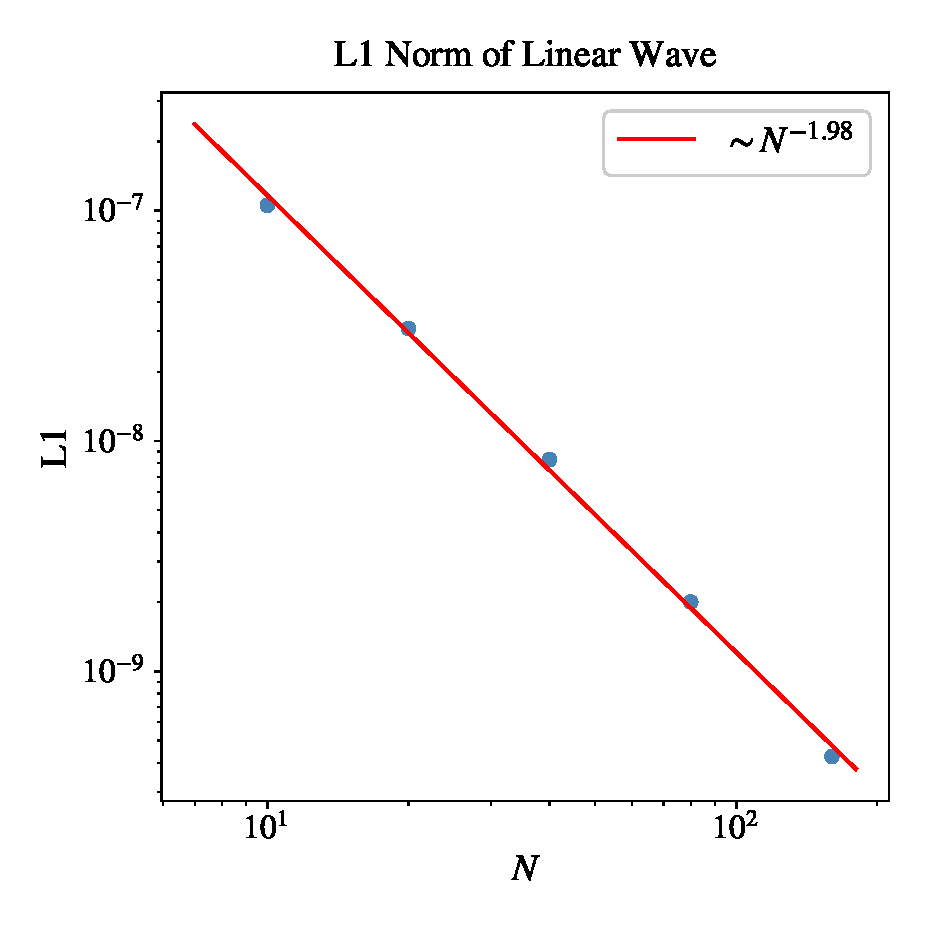
\includegraphics[width=0.4\textwidth]{figures/linear-wave-l1.eps}
        \caption{L1 norm of linear wave problem in 2d. Blue points are results
        of simulation from different resolutions overlaid by a linear fit showing
        the convergence is approximately second order. This example was produced by
        \textbf{linear\_wave\_2d.py} and \textbf{l1\_norm.py} scripts.}
        \label{fig.linear-wave}
    \end{center}
\end{figure}
Figure \ref{fig.linear-wave} shows the $L1$ norm as a function of grid cells per dimension.
As expected, the convergence rate is approximately second order in time and space for
this smooth problem. In the presence of shocks or other discontinuities it is not expected
to have such convergence.

\subsubsection{Sod shock-tube}
To examine the ability of the code to handle shock propagation we perform the Sod shock-tube 
problem \citep{toro-1997}. The problem consists of two different constant states at rest separated 
at the midpoint of the $x$ axis. A discontinuity exist in the density and pressure at that point. 
After $t=0$ the high density region flows into the lower density region. The flow produces a 
rarefaction, contact discontinuity, and a shock wave emanating from the density discontinuity. Thus, 
this problem creates a great test for the codes ability to capture the three wave types.

For our initial setup we use a unit box with reflective boundary conditions with density and pressure defined as
\begin{equation}
	\rho = \left\{
      \begin{array}{@{}ll@{}}
        	1.0 & \text{for}\ x \leq 0.5 \\
            0.125 & \text{for}\ x > 0.5
    	\end{array}\right.
\end{equation}
and
\begin{equation}
	P = \left\{
      \begin{array}{@{}ll@{}}
        	1.0 & \text{for}\ x \leq 0.5 \\
            0.1 & \text{for}\ x > 0.5
    	\end{array}\right.
\end{equation}
with $\gamma = 1.4$. The particles are laid out in a Cartesian grid and the simulation is evolved
until $t=0.15$. The number of particles per dimension is chosen to be $N=100$ and $N=45$ for 2D
and 3D respectively. This allows a comparison of a high and low resolution run.
\begin{figure}
    \begin{center}
        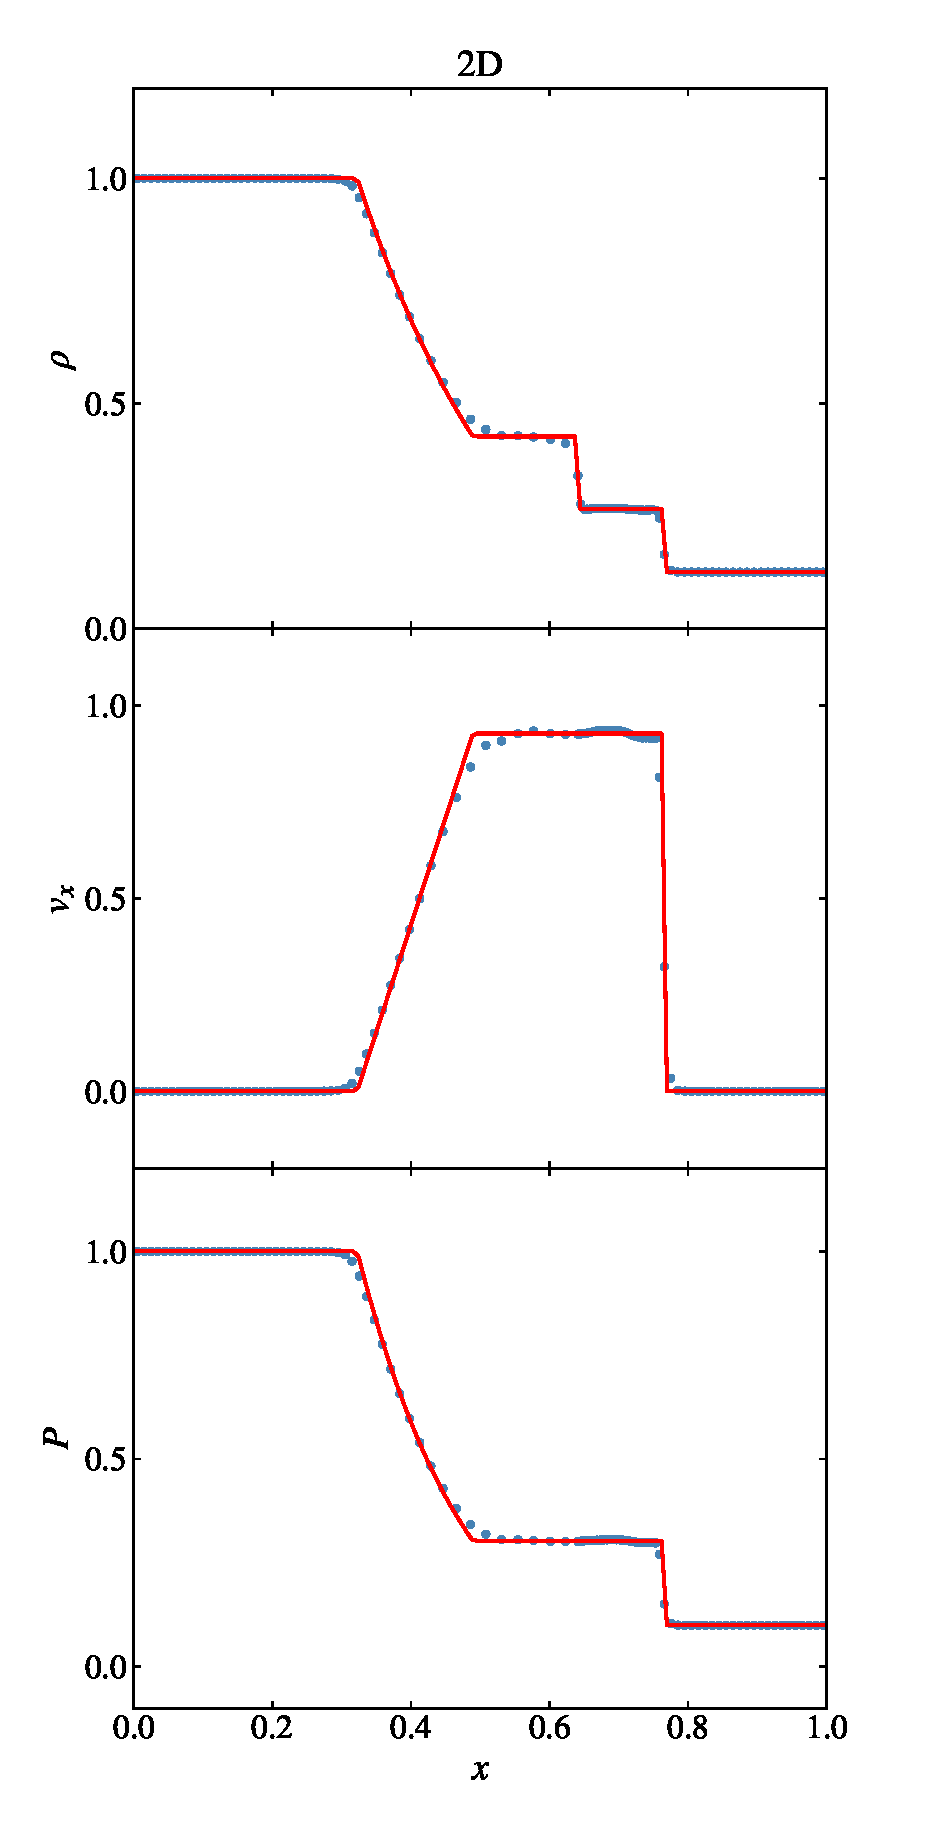
\includegraphics[width=0.4\textwidth]{figures/sod_2d.eps}
        \includegraphics[width=0.4\textwidth]{figures/sod_3d.eps}
        \caption{Profiles of density, $x$-component of velocity and pressure of the Sod 
        shock-tube simulation. Left: 2D run using a total of $100\times100$ particles. Right: 3D run 
        using a total of $45\times45\times45$, we only plot a slice of particles defined by $z=0$.
        Light blue points are the simulation while the red line is the exact solution.
        This example was produced by \textbf{sod\_2d\_cartesian.py},
        \textbf{sod\_3d\_cartesian.py}, \textbf{sod\_2d\_profiles.py}, and 
        \textbf{sod\_3d\_profiles.py} scripts.}
        \label{fig.sod}
    \end{center}
\end{figure}

Figure \ref{fig.sod} plots the particles density, $x$-component of velocity and pressure; only 
particles with $z=0$ are plotted in the 3D run for simplicity. The red line is the analytical 
solution. For the 2D simulation we can see the shock is well resolved as is the contact 
discontinuity. Further, the Lagrangian nature of the code can be seen as many particles have been 
squeezed between the contact discontinuity and the shock front while particles in the rarefaction 
have been spread out. For the 3D, lower resolution run, the code catches all three waves. Although, 
the contact discontinuity wave has been smoothed due to the lower number of particles.

\subsubsection{Explosion}
\begin{figure}
    \begin{center}
        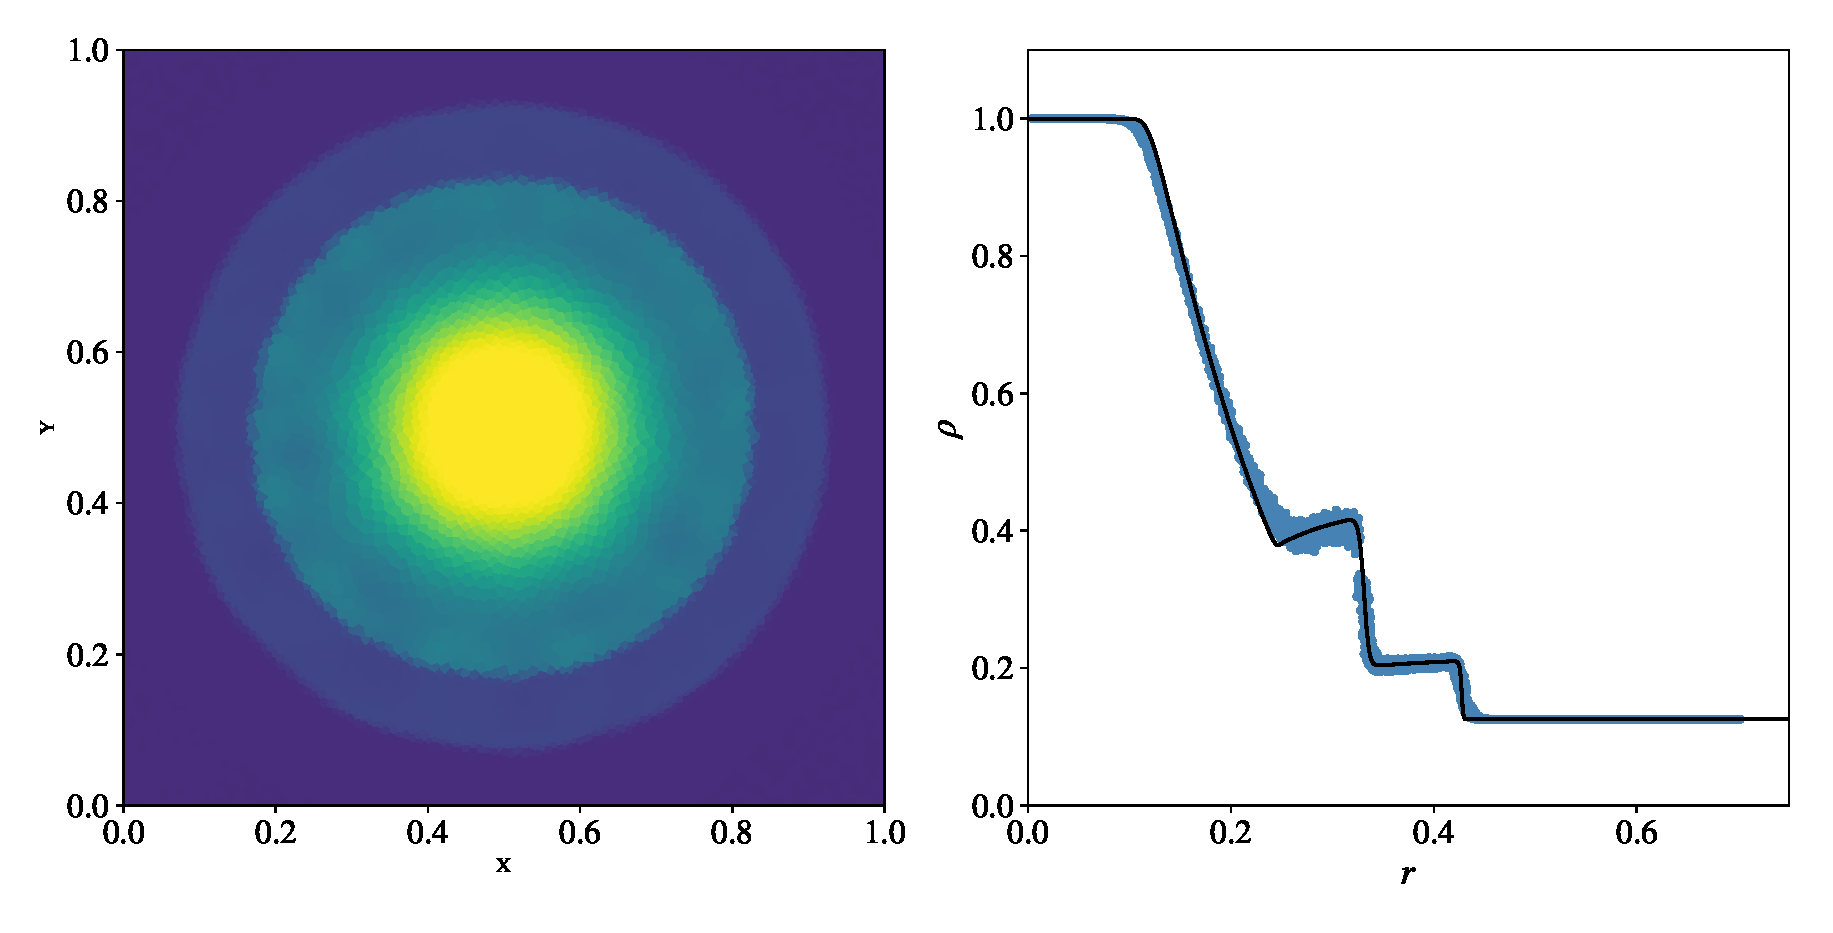
\includegraphics[width=0.8\textwidth]{figures/explosion_2d.eps}
        \caption{Density heatmap and radial profile of the Explosion problem. Left density
        heatmap, the irregular cells can been seen from the random initialization. Right
        radial density profile is an agreement with the exact solution in red.
        This example was produced by \textbf{explosion\_2d\_random.py} and 
        \textbf{explosion\_density\_panel.py} scripts.}
        \label{fig.explosion_2d}
    \end{center}
\end{figure}
An analog to the Sod problem is the 2D explosion problem \citep{toro-1997}. Like the Sod problem, 
the domain is partitioned into two constant states. However, the higher density region is now a 
circular region of radius $r$ centered in a unit box. Similar to the Sod problem, the initial 
conditions generate a shock, contact discontinuity and rarefaction wave. However, in this case
the waves are now a circular shock traveling radially outward, a circular contact
discontinuity traveling in the same direction, and a rarefaction wave traveling towards the
center.

We use the same values as the Sod problem except we restrict the higher density values onto
the center of domain with radius $r=0.25$. Further, instead of using a Cartesian grid we sample
particles uniformly for a unit square and perform 10 iterations of Lloyds algorithm. 

Figure \ref{fig.explosion_2d} shows the density map and density profile. Clearly, the cells
density matches the analytical solution in red. Further, the solution captures all three waves
even though the mesh was built in a random fashion. This an important difference over Eulerian
codes, since Lagrangian codes are not constrained to any initial particle placement. Therefore
one can reach better accuracy by placing the particles in way that exploits the problem. We will
see a later example of this in the Evrards problem, see Section \ref{sec.evrards}.

\subsubsection{Gresho vortex}
Our next problem will test stability of the code in maintaining equilibrium. \cite{Gresho90}, 
introduced an interesting problem to test for conservation of angular momentum. A vortex in a unit 
2D box with constant density $\rho=1$ is setup with the following angular velocity
\begin{equation}
	v_\phi (r) = \left\{
      \begin{array}{@{}ll@{}}
        	5r & \text{for}\ 0 \leq r < 0.2 \\
            2-5r & \text{for}\ 0.2 \leq r < 0.4 \\
            0 &\text{for}\ \geq 0.4
    	\end{array}\right.
\end{equation}
The angular velocity of the vortex grows linearly as one moves radially outward from
the center until midway of the disk. Then the velocity decreases linearly until it
vanishes at the rim of the disk. This produces triangular shape velocity profile.
The corresponding pressure is
\begin{equation}
	P(r) = \left\{
      \begin{array}{@{}ll@{}}
        	5 + 25/2r^2 & \text{for}\ 0 \leq r < 0.2 \\
            9+25/2r^2 - 20r + 4\ln(r/0.2) & \text{for}\ 0.2 \leq r < 0.4 \\
            3 + 4\ln(2) &\text{for}\ \geq 0.4.
    	\end{array}\right.
\end{equation}
The pressure is chosen such that the pressure gradients balance the centrifugal forces
generated by the rotation. Thus producing a solution that is independent of time.
\begin{figure}
    \begin{center}
        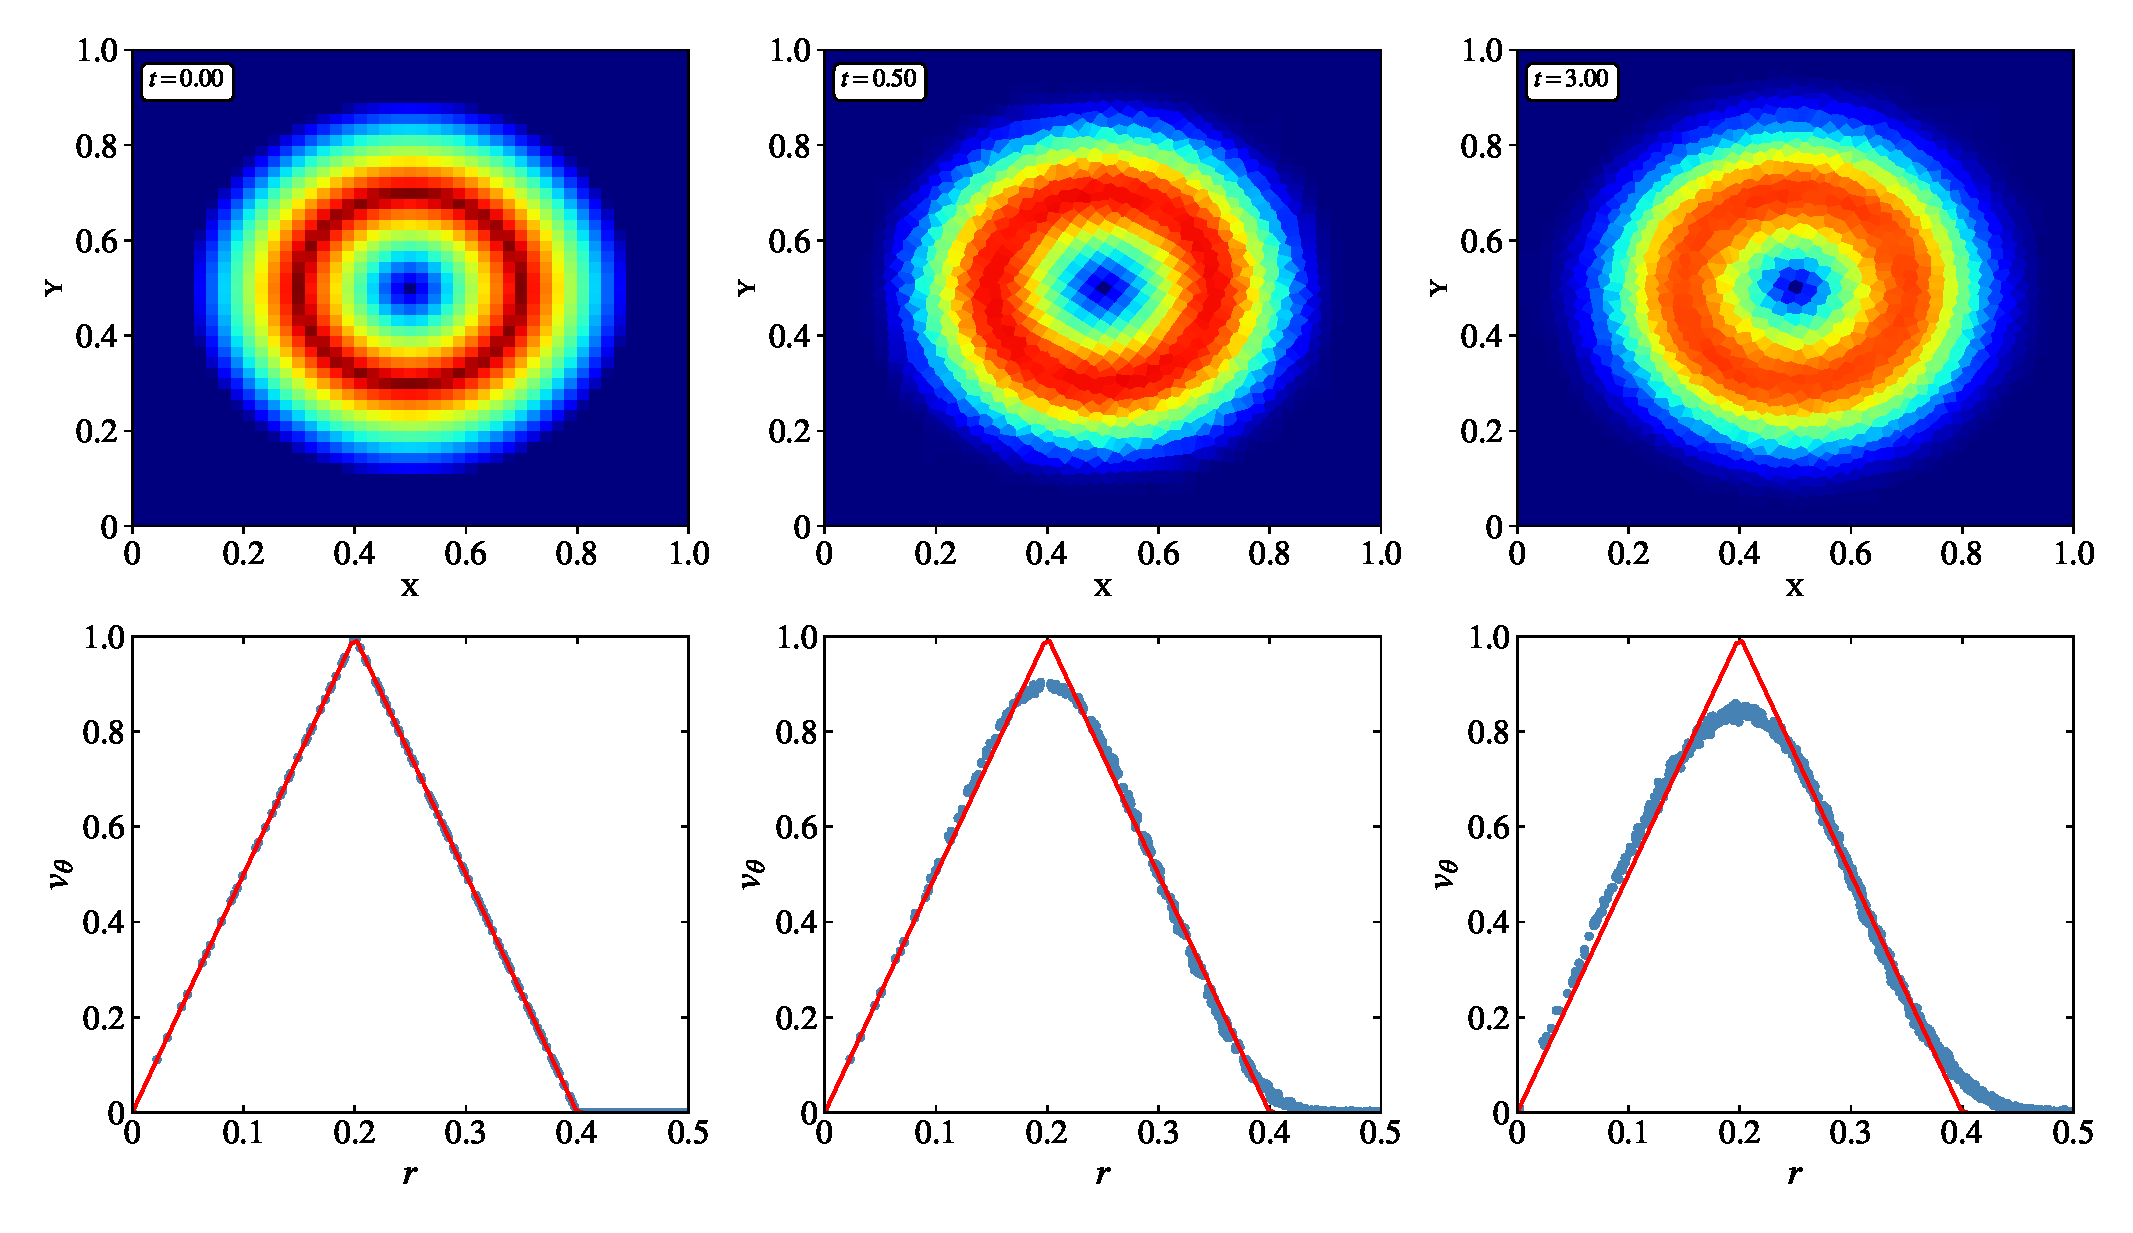
\includegraphics[width=0.8\textwidth]{figures/gresho_vortex.eps}
        \caption{Heatmap and radial profile of azimuthal velocity. Top row: time evolution
        of the cells at times $t=0.0, 0.5, 3.0$. Bottom row: corresponding radial profile of 	
        azimuthal velocity. As the simulation evolves the systems remains in equilibrium.
        This example was produced by \textbf{gresho\_2d\_cartesian.py} and 
        \textbf{gresho\_density\_panel.py} scripts.}
        \label{fig.gresho_vortex}
    \end{center}
\end{figure}
Figure \ref{fig.gresho_vortex} shows three snapshots at $t=0.0, 0.5, 3.0$ of the azimuthal
velocity. The top row is a 2d heat map while the bottom row is a radial profile. At time $t=0$
all the cells are rectangular. As the system evolves the cells that are rotating become irregular 
polygons. There is a small amount of velocity smoothing at the initial largest velocities and at
the rim of the vortex. However, it is evident that the system stays in equilibrium.

\subsubsection{Sedov-Taylor}
Another test that generates a shock is the Sedov-Taylor blast wave problem \citep{Sedov1959}. In 
this problem a homogeneous gas is injected with a large amount of energy in a point-like region at 
the center of the domain. A spherical shock is created emanating from the center. The shock 
propagates radially outward sweeping mass into a thin shell and creating a cavity behind the shock. 
The problem has a well known analytical self-similar solution; see \cite{Sedov1959} for details. 
Applying the Rankine–Hugoniot at the shock front the density jumps to a maximum compression of
\begin{equation}
	\rho_{\mathrm{max}}/\rho = (\gamma + 1)/(\gamma - 1),
\end{equation}
for $\gamma = 5/3$ this amounts to a max value of 4.

We consider the 2D and 3D case. A unit box is setup with particles in a Cartesian grid of size
$45\times 45$ and $45 \times 45 \times 45$ for 2D and 3D respectively. The stationary gas has
a constant density of $\rho = 1.0$ and pressure $P = 10^{-6}$ with $\gamma=5/3$. The simulation is
allowed to evolve to time $t=0.06$.
\begin{figure}
    \begin{center}
        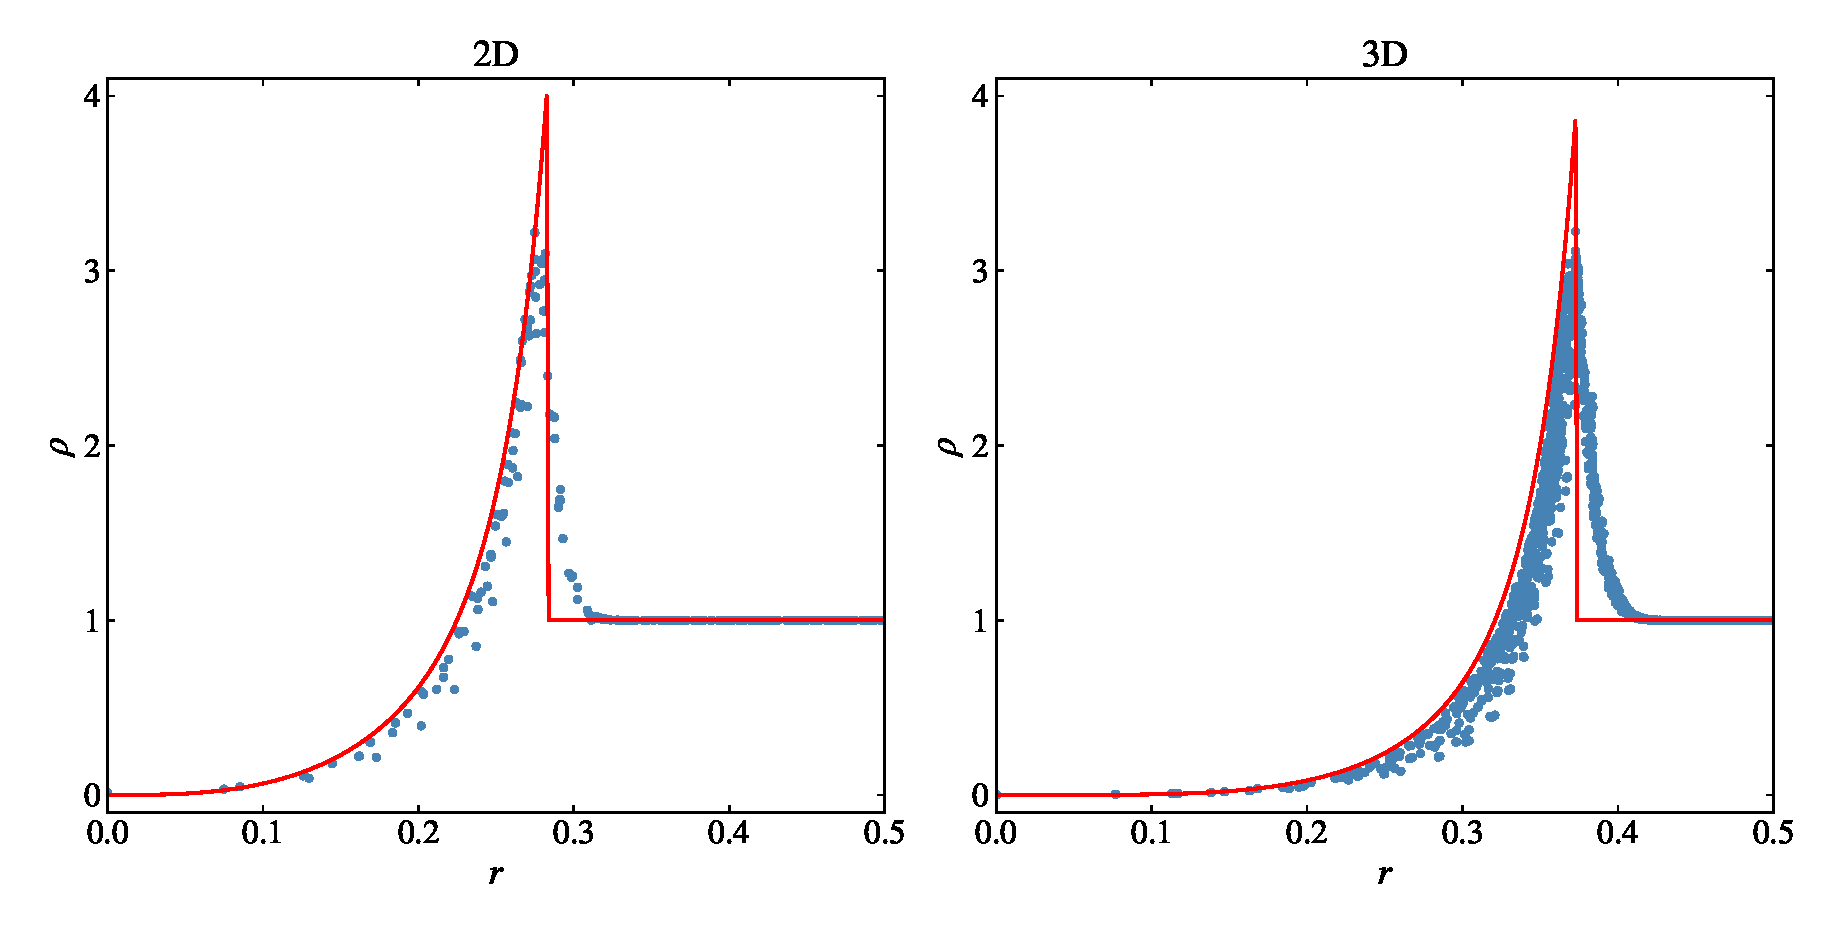
\includegraphics[width=0.8\textwidth]{figures/sedov_compare.eps}
        \caption{Density profile of Sedov-Taylor blast wave problem. Left: 2D version with an 
        initially Cartesian mesh of $45 \times 45$. Right: 3D version with an initially 
        Cartesian mesh of $45 \times 45 \times 45$; only a random sample of $45\times45$ is
        plotted for simplicity. Light blue points are the density at radius $r$ 
        from the center of the explosion while the red line is the exact solution.
        This example was produced by \textbf{sedov\_2d\_cartesian.py},
        \textbf{sedov\_3d\_cartesian.py}, and \textbf{sedov\_density\_compare.py} scripts.}
        \label{fig.sedov}
    \end{center}
\end{figure}
Figure \ref{fig.sedov} shows the cell density as a function of radial distance from the center of 
the explosion. It is noted that shock is well resolved by the cells as the mesh has deformed in such 
a way that the shock front contains a large amount of cells which is evident in
Figure \ref{fig.sedov_panel}.
\begin{figure}
    \begin{center}
        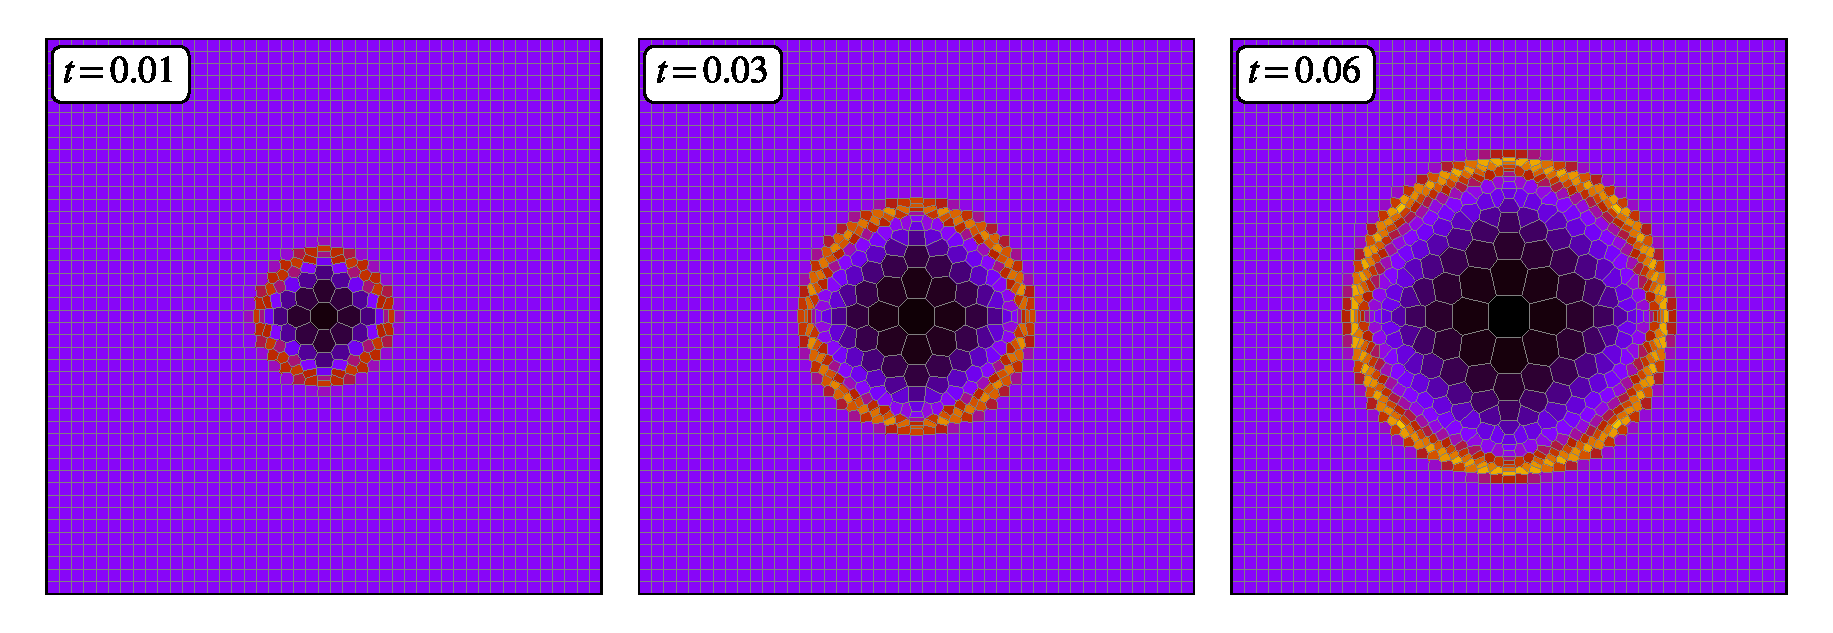
\includegraphics[width=0.8\textwidth]{figures/sedov_panel.eps}
        \caption{Evolution of the density at several times. The initial cell with the energy
        imparted remains stationary as the cells around it move radially outward. The cells at
        the shock are compressed allowing for better resolution. This example was produced by 
        \textbf{sedov\_2d\_cartesian.py} and \textbf{sedov\_density\_panel.py} scripts.}
        \label{fig.sedov_panel}
    \end{center}
\end{figure}
The center cell, where the energy is deposited, remains stationary while the
cells around it move radially outward. The cells exterior to the shock remain
stationary until they are swept and compressed by the shock.

\subsubsection{Kelvin-Helmholtz instability}
For our last hydrodynamic test we consider the Kelvin-Helmholtz (KH) instability. This
problem consist of a shear-flow where a single mode is excited by a velocity perturbation.
Specifically, two layers with different densities are initially in pressure equilibrium. 
Each layer flows in the opposing direction and receives a velocity perturbation perpendicular
to the interface. The perturbation grows exponentially and produces structures which
are called KH instabilities. A difficulty of this problem is that
numerical errors, noise, and resolution seed spurious small structure \citep{Lecoanet2016}
making direct comparisons a difficult endeavor. However, we can use this problem to
visually verify the characteristics of the problem are maintained
and leave the exact detail treatment to the next revision of the code.

We follow \cite{Springel2010} and setup a unit periodic box with density
\begin{equation}
	\rho = \left\{
      \begin{array}{@{}ll@{}}
            2 & \text{for}\ y < 0.25 \\
            1 & \text{for}\ 0.25 \leq y \leq 0.75\\
            2 & \text{for}\ 0.75 < y,
    	\end{array}\right.
\end{equation}
$x$-component of velocity
\begin{equation}
	v_x = \left\{
      \begin{array}{@{}ll@{}}
            -0.5 & \text{for}\ y < 0.25 \\
            0.5 & \text{for}\ 0.25 \leq y \leq 0.75\\
            -0.5 & \text{for}\ 0.75 < y,
    	\end{array}\right.
\end{equation}
and $y$-component of velocity
\begin{equation}
	v_y(x, y) = w_0 \mathrm{sin}(4\pi x) \left(\exp\left(-\frac{(y-0.25)^2}{2\sigma^2}\right) +
    	\exp\left(-\frac{(y-0.75)^2}{2\sigma^2}\right)\right)
\end{equation}
where $w_0=0.1$ and $\sigma=0.05/\sqrt{2}$. The pressure is set to $P=2.5$, $\gamma=5/3$
and the simulation is evolved until time $t=2$.
\begin{figure}
    \begin{center}
        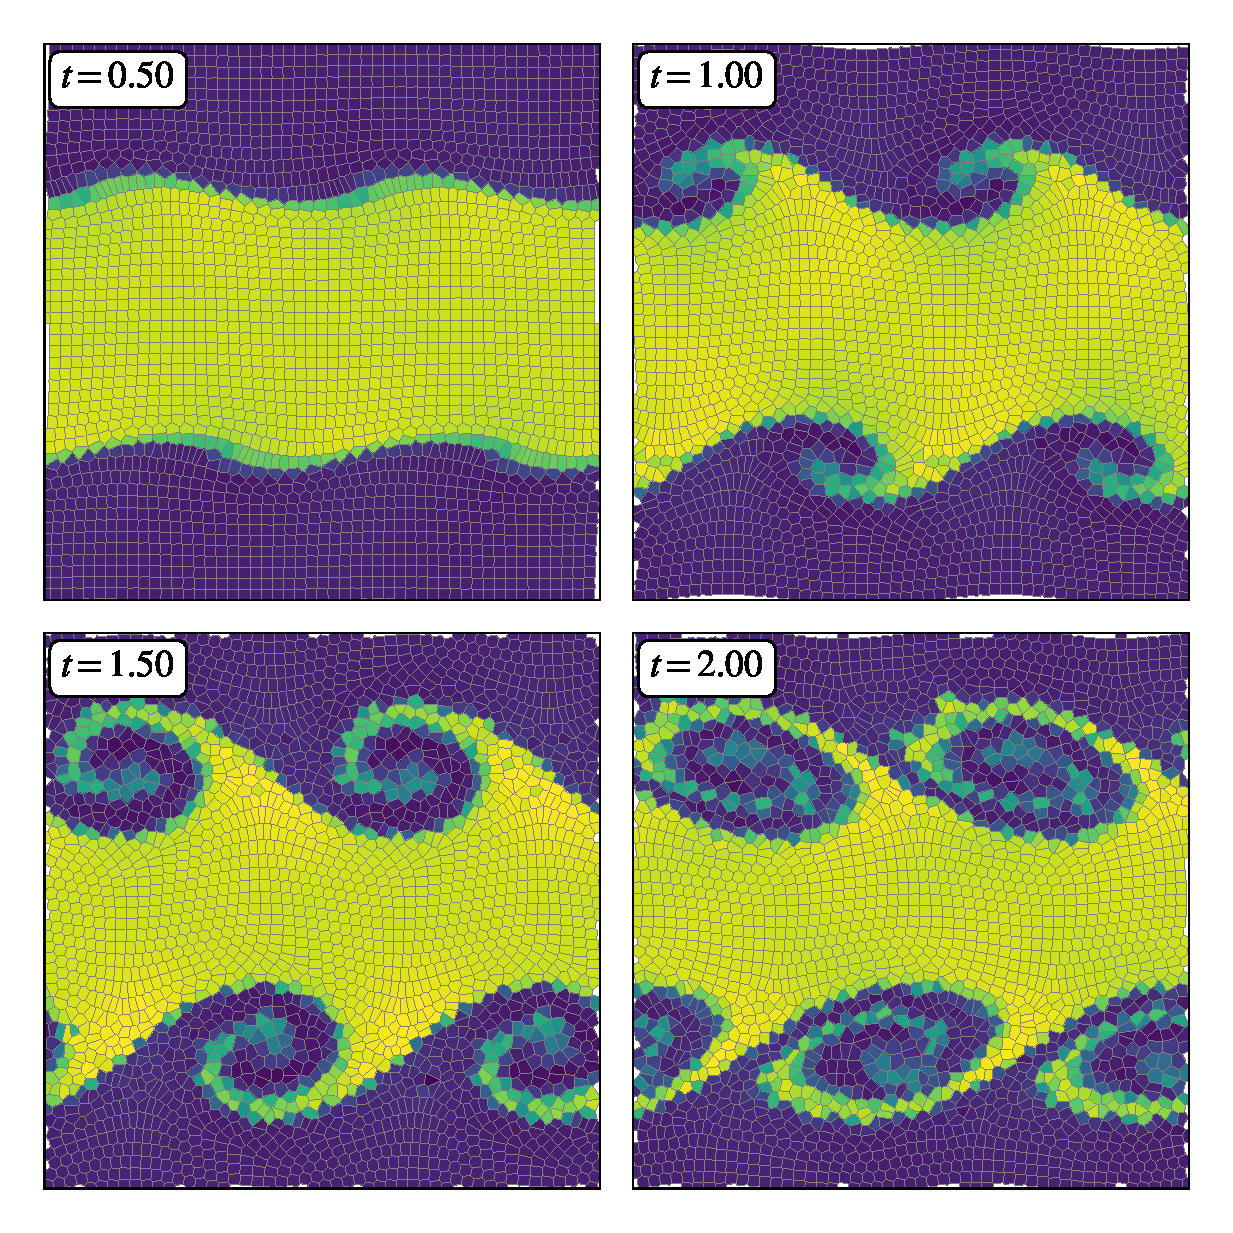
\includegraphics[width=0.8\textwidth]{figures/kelvin.eps}
        \caption{Evolution of the density at several times in the KH problem. We see the common
        traits of KH evolution, KH billows and mixing. This example was produced by 
        \textbf{kelvin\_helmholtz\_2d\_cartesian.py} and 
        \textbf{kelvin\_helmholtz\_density\_panel.py} 
        scripts.}
        \label{fig.kelvin}
    \end{center}
\end{figure}

Figure \ref{fig.kelvin} shows the density field for several selected times. Comparing with
Springel, visually we conclude that the results are in close agreement. The formation of the
Kevlin Helmholtz billows and mixing of both fluids at each time are similar.

\subsection{Gravity Tests}
\subsubsection{Two body}
Our first problem, in testing our gravity solver, is a simple two body problem where two particles
interact with each other through their gravitational force. Although, this problem does not really test the 
implementation of the gravity tree, since only two leaves will be constructed
in the tree and it is most likely that the leaves will interact with each other bypassing the node 
moments, it does test the gravity kernel and stability of the leap frog integrator.

For this problem an exact solution exists by reducing it to a single body. Given
two particles with masses $m_1$ and $m_2$ with positions $\vec{r}_1$ and $\vec{r}_2$ the equation of motion for
the reduced mass
\begin{equation}
	\frac{1}{\mu} = \frac{1}{m_1} + \frac{1}{m_2}
\end{equation}
is
\begin{equation}
	\mu\frac{d^2 \vec{r}}{dt^2} = -\frac{G m_1 m_2}{r^2}\hat{r},
    \label{eq.reduced-force}
\end{equation}
where $\vec{r}$ is the separation vector $\vec{r}_1 - \vec{r}_2$. Equation \ref{eq.reduced-force} can be
transformed to polar coordinates giving the solution
\begin{equation}
	r = \frac{a(1-\epsilon^2)}{1-\epsilon cos(\theta)}
\end{equation}
for initial conditions $a$ and $\epsilon$. The overall system evolves with a period of
\begin{equation}
    T = \sqrt{\frac{4\pi^2 a^3}{G m}},
\end{equation}
where $m=m_1 + m_2$. To recover the particles positions, a final transformation
of the form
\begin{equation}
	\begin{array}{rcl}
		\vec{r}_1 & = & \frac{m_1}{m}\vec{r}\\
    	\vec{r}_2 & = & -\frac{m_2}{m}\vec{r}
    \end{array}
\end{equation}
is used. The initial position and velocity of the particles can be parameterized by $a$,
$\epsilon$ and $q=m_1/m_2$
\begin{equation}
	\begin{array}{rcl}
    	\vec{r}_1 & = & a\frac{1-\epsilon}{1+q} \hat{x}\\
        \vec{v}_1 & = & \frac{1}{1+q}\sqrt{\frac{1+\epsilon}{1-\epsilon}}\sqrt{\frac{Gm}{a}} \hat{y}\\
        \vec{r}_2 & = & -q \vec{r}_1\\
        \vec{v}_2 & = & -q \vec{v}_1.
    \end{array}
\end{equation}

We setup the particles with parameter values $a=0.5$ and $\epsilon=0.25/0.75$ with $G=1$ and allow
the simulation to evolve for 10 periods. The time step is held fixed with a value of $dt=T/1000$.
In Figure \ref{fig.two_body} we show the trajectory for both particles as well as the evolution of
the relative total energy error. We clearly see that both trajectories remain along the exact solution
signifying the stability of the leap frog integrator. Further we see that the relative total energy
error remains bounded by zero and $-1.1\times10^{-4}$ indicating that the total energy remains
accurately conserved.
\begin{figure}
    \begin{center}
        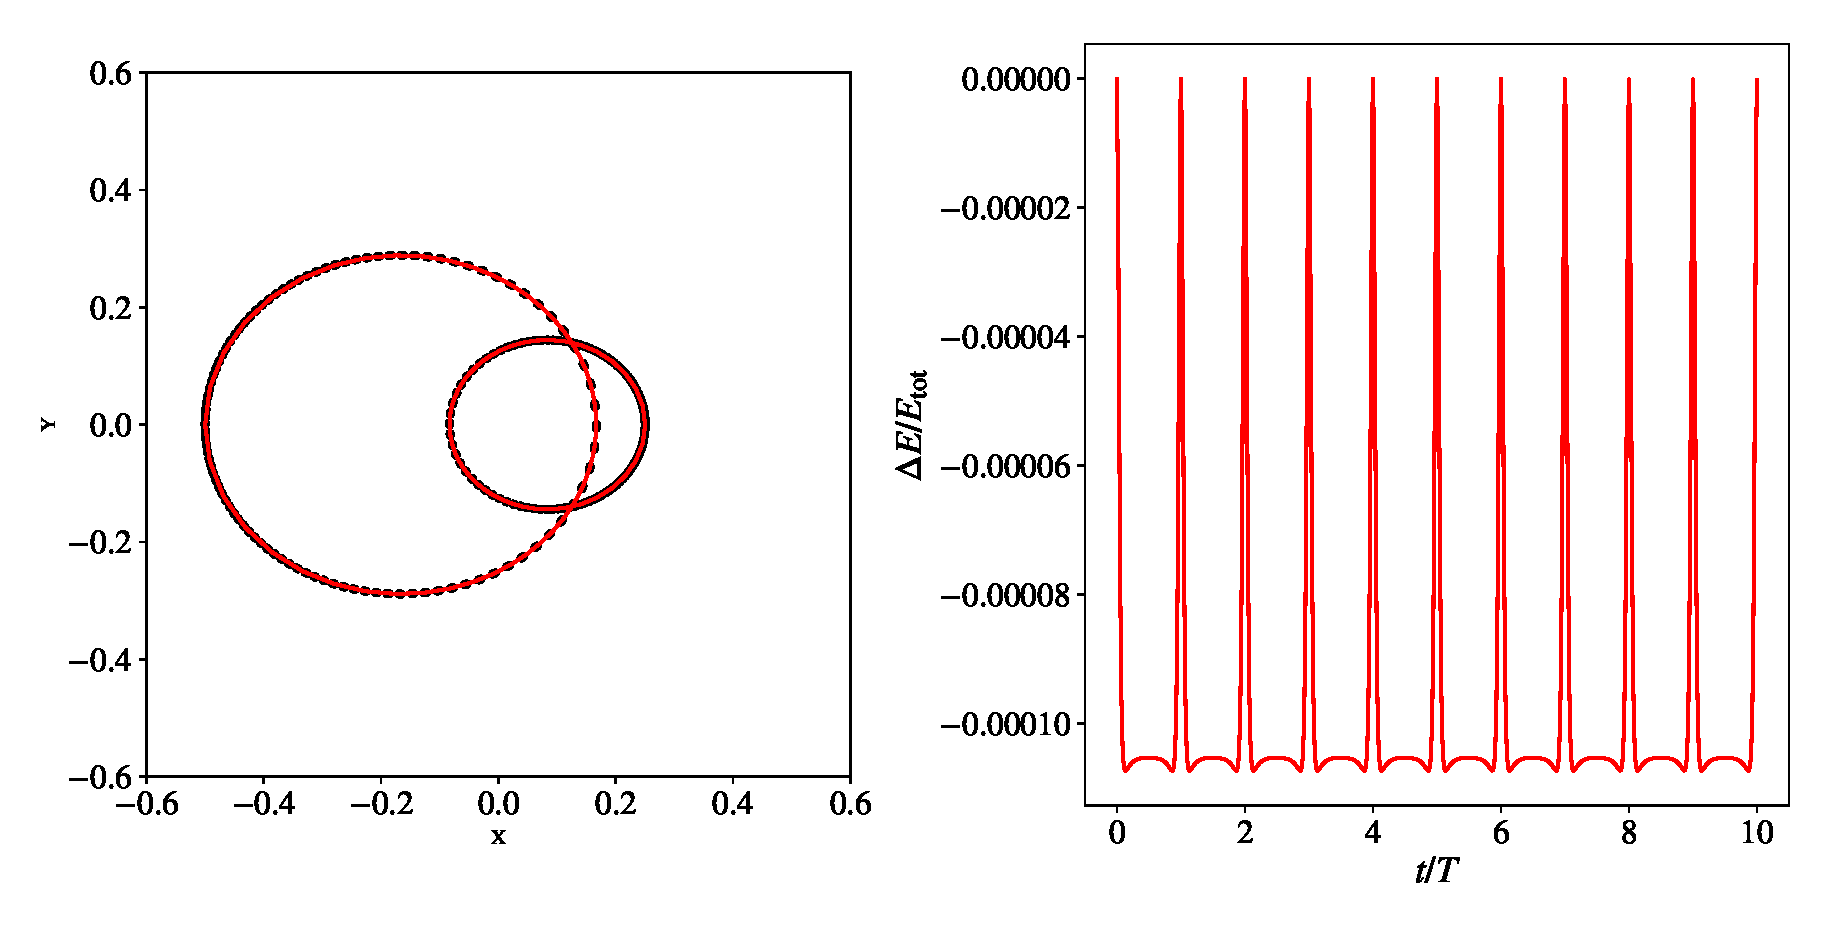
\includegraphics[width=0.9\textwidth]{figures/two_body.eps}
        \caption{Left: Trajectories of the two body problem for ten periods. Clearly
        both particles remain in their orbital path shown in red signifying the stability
        of the leap frog integrator. Right: Corresponding relative total energy error.
        The total energy remains accurately conserved as the worst relative error is
        $-1.1\times10^{4}$.}
        \label{fig.two_body}
    \end{center}
\end{figure}

\subsubsection{Plummer sphere}
The Plummer sphere cite is a model that can be used to describe the distribution of stars and in a cluster
and is commonly used to test gravity solvers. The Plummer sphere, i.e. a polytrope of index 5,
has a density profile of the from
\begin{equation}
	\rho (r) = \frac{3 M}{4\pi R^3} \left(1 + (r/R)^2\right)^{-5/2},
    \label{eq.plummer}
\end{equation}
where $M$ is the total mass of the cluster and $R$ is a scale parameter which sets the
size of the cluster. The system is in steady state with an isotropic velocity distribution.
To test our gravity solver, we initialize our particles with the given distributions and
advance the system in time. We expect the system to stay in steady state therefore we compare
the initial density distribution with the final state of the system.

For our test we chose the parameters of the Plummer sphere to be $M=1,000$ and $R=1$ with
$G=1$. We then sampled 10,000 particles using the the rejection technique outlined in
cite to set the position and velocities. The system is allowed to evolve to time $t=1$
which is roughly ten dynamical times. The gravitational tree used an opening angle 0.4
and smoothing parameter of 0.03.
\begin{figure}
    \begin{center}
        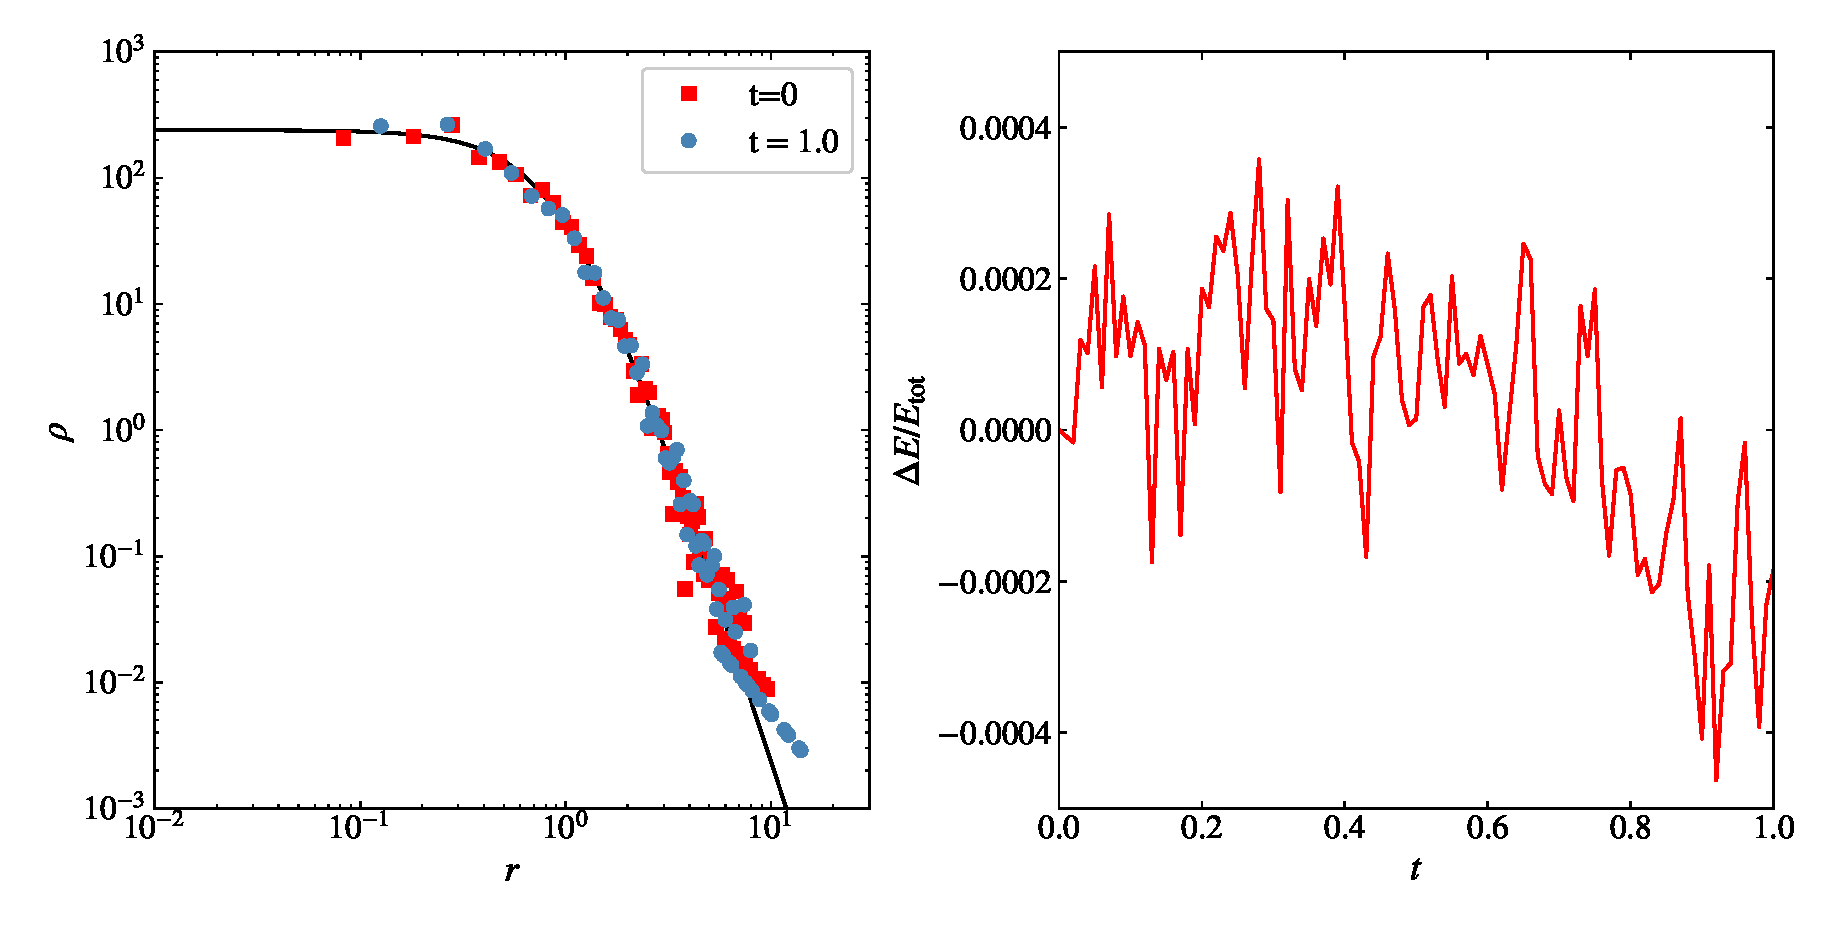
\includegraphics[width=0.9\textwidth]{figures/plummer.eps}
        \caption{Density profile of Sedov-Taylor blast wave problem. Left is the 2D version with an initially
        Cartesian mesh of $45 \times 45$. Right is the 3D version with an initially Cartesian mesh of 
        $45 \times 45 \times 45$. Light blue points are the density a radius $r$ from the center of the explosion
        while the red line is the exact solution.}
        \label{fig.plummer}
    \end{center}
\end{figure}
The left panel of Figure \ref{fig.plummer} shows the density profile at the initial and final 
time of the simulation with equation \ref{eq.plummer} overlaid as a reference. The density is calculated
by dividing the space by spherical shells, binning and dividing by the volume. It is clearly shown that
at the final time the particles remain in steady state with their positions matching the initial
distribution. The right panel of \ref{fig.plummer} shows the evolution of the relative error of the
total energy of the system. The error stays well below $5\times 10^{-4}$ with a final error of
$2\times 10^{-4}$, entailing the solver has accurately maintained the total energy.

\subsubsection{Rayleigh Taylor}
Our first hydrodynamic problem to include gravity is the Rayleigh Taylor instability problem.
The problem consists of dense fluid over a lighter fluid in the presence of a uniform 
vertical gravitational field. A perturbation is placed in the vertical direction causing the
dense field to sink while the lighter rises through buoyancy.

A rectangular domain of the size $[1\times3]$ is chosen with the gravitational force in the
$y$-direction with strength of $g=1$. The initial setup of the density
is
\begin{equation}
	\rho = \left\{
      \begin{array}{@{}ll@{}}
            1 & \text{for}\ y \leq 1.5 \\
            2 & \text{for}\ 5 > 1.5,
    	\end{array}\right.
\end{equation}
while the pressure is
\begin{equation}
	P = \left\{
      \begin{array}{@{}ll@{}}
            10 - y & \text{for}\ y \leq 1.5 \\
            11.5 + 2(y-1.5) & \text{for}\ 5 > 1.5,
    	\end{array}\right.
\end{equation}
such that the system is initially in hydrostatic equilibrium. A perturbation is applied
to the $y$-velocity
\begin{equation}
	v_y = \mathrm{cos}\left(2\pi x\right)\exp{-(y-1.5)^2/0.1}
\end{equation}
We set $\gamma=1$ and let the system evolve to $t=3.0$. Although without an implementation
of viscosity there is no one correct solution that all codes converge to. However, we can
visually inspect if our simulation share the same characteristics of another established
code. In Figure we that the single mode is very similar to the results from cite
\begin{figure}
    \begin{center}
        \includegraphics[width=0.6\textwidth]{figures/rayleigh_compare.eps}
        \caption{Density profile of Sedov-Taylor blast wave problem. Left is the 2D version with an initially
        Cartesian mesh of $45 \times 45$. Right is the 3D version with an initially Cartesian mesh of 
        $45 \times 45 \times 45$. Light blue points are the density a radius $r$ from the center of the explosion
        while the red line is the exact solution.}
        \label{fig.rayleigh}
    \end{center}
\end{figure}

We see the mode has the characteristics of

\subsubsection{Evrard Collapse}
\label{sec.evrards}
The final test is the Evrards collapse problem which tests the coupling of self-gravity and hydrodynamics.
The problem consists of an initially non-rotating isothermal gas sphere with mass $M=1$ and radius $R=1$
with a density 
\begin{equation}
	\rho(r) = \left\{
      \begin{array}{@{}ll@{}}
            1/\left(2\pi r\right) & \text{for}\ r \leq 1 \\
            0 & \text{for}\ r > 1
    	\end{array}\right.
\end{equation}
and pressure
\begin{equation}
	P(r) = \left\{
      \begin{array}{@{}ll@{}}
            0.05 /\left(3\pi r\right) & \text{for}\ r \leq 1 \\
            0 & \text{for}\ r > 1.
    	\end{array}\right.
\end{equation}
The gravitational constant is set to $G=1$ and $\gamma=5/3$. The evolution of the sphere begins
with mass falling towards the center due to self-gravity. The pressure at the center rises and
produces a shock traveling outward through the in-falling gas. The final state of the gas is a
spherical distribution in hydrostatic virial equilibrium.

We setup an initial Cartesian grid of size $33\times 33\times 33$ particles. Due to the nature
of the $1/r$ density profile, a Cartesian mesh will not resolve the high density values unless
the resolution is sufficiently increased. However we have complete freedom on how to the particles
are initially setup. Therefore, we transform particles radially inside the sphere by the following
\begin{equation}
    r_{\mathrm{new}} = r_{\mathrm{old}}^{3/2}.
\end{equation}
Such a transformation maps a grid of equally spaced particles with uniform density to
a set of particles spaced in such a way that the uniform density follows a $1/r$ profile. 
\begin{figure}
    \begin{center}
        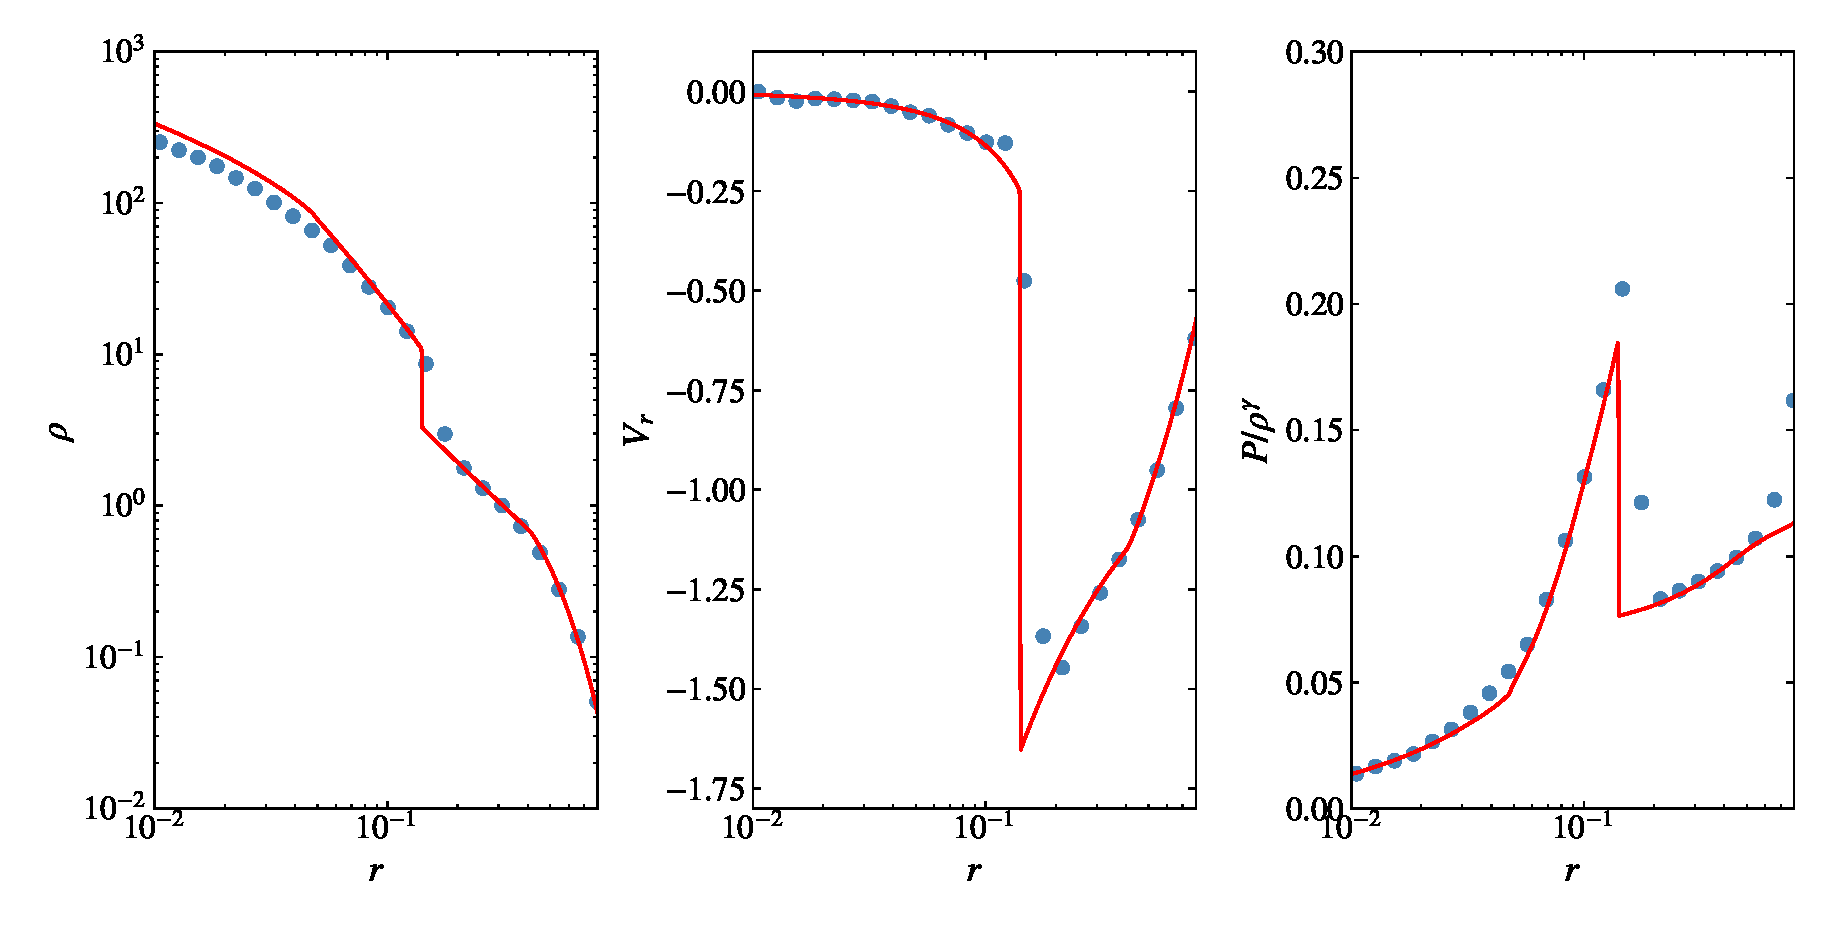
\includegraphics[width=0.9\textwidth]{figures/evrard.eps}
        \caption{Density profile of Sedov-Taylor blast wave problem. Left is the 2D version with an initially
        Cartesian mesh of $45 \times 45$. Right is the 3D version with an initially Cartesian mesh of 
        $45 \times 45 \times 45$. Light blue points are the density a radius $r$ from the center of the explosion
        while the red line is the exact solution.}
        \label{fig.evrard}
    \end{center}
\end{figure}

The radial averaged density, radial velocity and entropy are shown in Figure at time $t=0.81$
when the shock has formed and is traveling outward. We see all profiles adequately follow the
exact solution in red for this low resolution run. Further we see that there is significant
error in the conservation of energy Figure. This is expected as noted by Springel. The 
discrepancy arises from the gravitational work term which ignores the motion of mass
exchanged by adjacent cells. Springel proposed a new formulation for then energy equation
that results in better energy conservation. This updated method will be added in the next
revision of the code.
\begin{figure}
    \begin{center}
        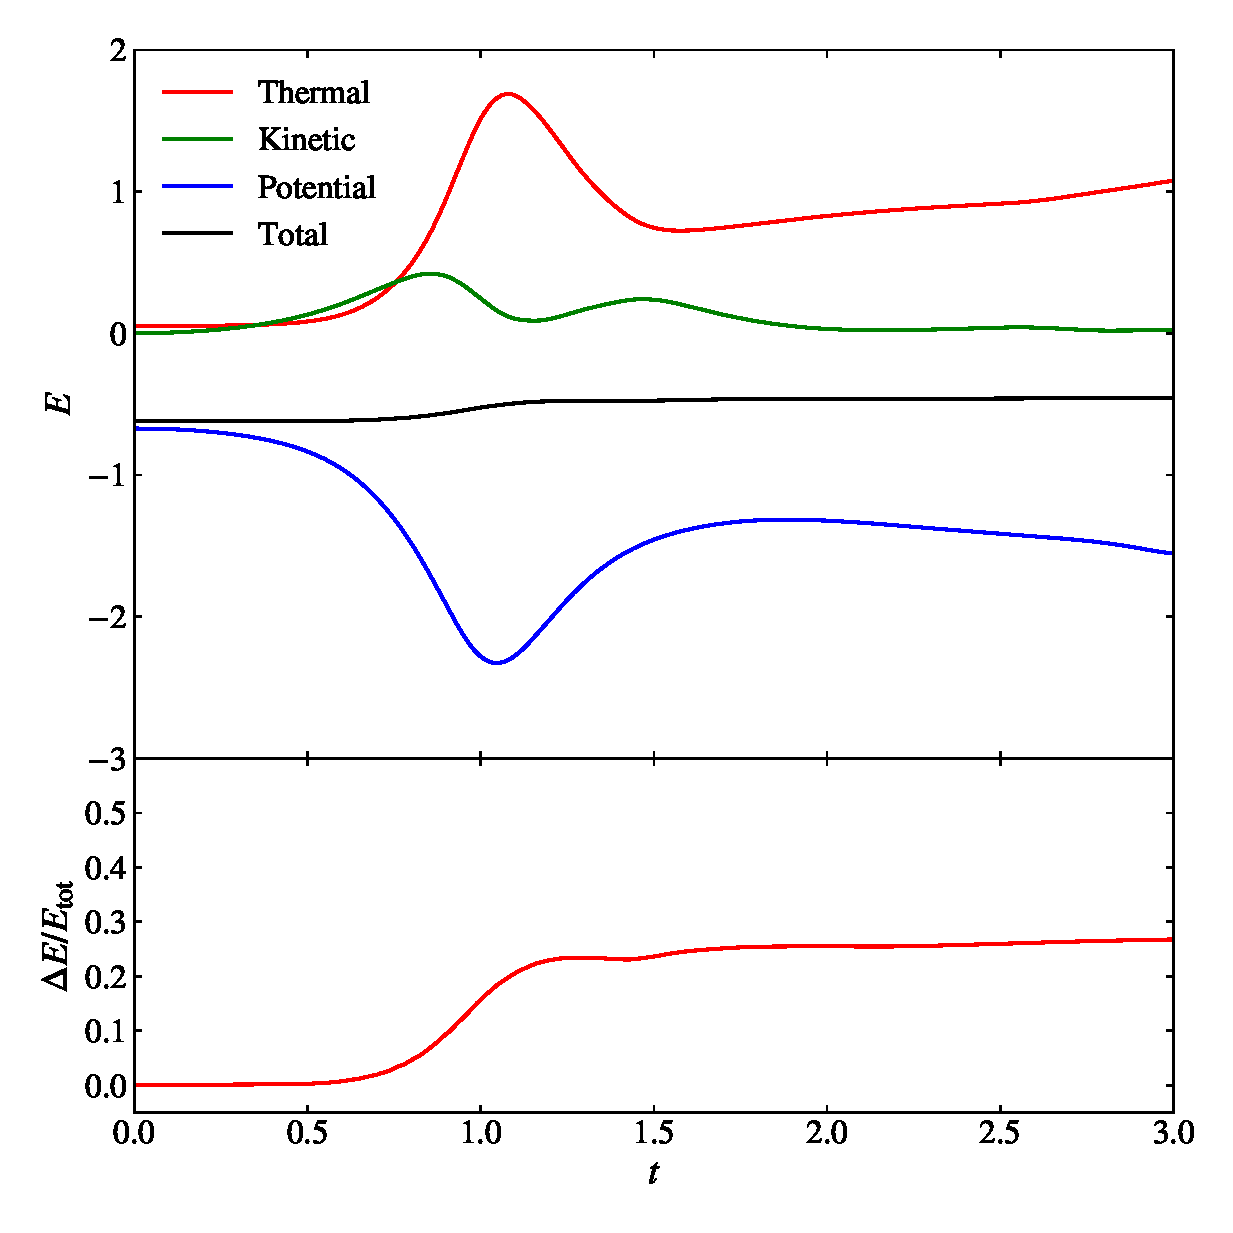
\includegraphics[width=0.6\textwidth]{figures/evrard_energy.eps}
        \caption{Density profile of Sedov-Taylor blast wave problem. Left is the 2D version with an initially
        Cartesian mesh of $45 \times 45$. Right is the 3D version with an initially Cartesian mesh of 
        $45 \times 45 \times 45$. Light blue points are the density a radius $r$ from the center of the explosion
        while the red line is the exact solution.}
        \label{fig.evrard_energy}
    \end{center}
\end{figure}


% Section: conclusions
%%%%%%%%%%%%%%%%%%%%%%%%%%%%%%%%%%%%%%%%%%%%%%%%%%%%%%%%%%%%%%%%%%%%%%%%%%%%%%
\section{Conclusions}
\label{sec.conclusions}

In this paper, we have presented the algorithms underlying \enzo, an
open-source adaptive mesh refinement code designed for
self-gravitating compressible fluid dynamics, including the effects of
magnetic fields, radiation transport, and a variety of microphysical
and subgrid processes.  In addition, we have described the \enzo\ code
development process, have shown the outputs of a set of representative
test problems, and have provided information about \enzo's performance
and parallel scaling on recent supercomputing platforms.  The \enzo\
code, its test suite, and all of the scripts used to generate plots
and figures for this paper are open source and are available at the
\enzo\ website, \url{http://enzo-project.org}.  Furthermore, the
\texttt{yt} toolkit, which is designed to analyze \enzo\ data (as well
as data from a wide variety of other simulation tools), can be found
at its website, \url{http://yt-project.org}.  Both of these codes have
active user and developer communities, extensive documentation and
user support, and strong mechanisms for users to contribute their
changes and fixes to the codebase.

The developers of the \enzo\ code are currently working on several
projects that will extend the functionality, scalability, or overall
performance of the code in the near future.  Projects that will appear
in forthcoming releases of the \enzo\ code include:

\begin{itemize}
\item The creation of a hybrid-parallel version of \enzo, combining
MPI for communication between nodes of a supercomputer and OpenMP for
thread-based parallelism within a node.  This will reduce on-node
memory usage and improve overall scaling behavior.
\item The restructuring of \enzo's treatment of particles to
accommodate a wider range of ``active'' particles that can easily
interact with each other and with multiple grids, and include sink,
source, and particle creation, destruction, splitting, and merging
functionality.
\item A new HYPRE-based AMR gravity solver that is faster, more
accurate, and more scalable than the current multigrid solver.
\item New infrastructure for problem initialization, enabling users to
more quickly and easily create new types of simulations.
\end{itemize}

With the continual rapid development of computer hardware, it makes
sense to not only review \enzo's current capabilities, but to look
toward its future development in view of predicted technological
trends. These trends in supercomputing hardware suggest that
substantial modifications to \enzo's core infrastructure, and very
possibly some of the core algorithms, will be required. More
specifically, the progression involves the usage of specialized
large-core-count, vectorized computing units such as graphics
processing units or chips like the Intel Xeon Phi, as well as
precipitously decreasing amounts of RAM per computing core.  The
former trend means that the amount of processing power per compute
node will continue to increase, likely much faster than the bandwidth
between nodes, and will require tremendous reduction in inter-node
(and possibly inter-CPU) communication in order to maintain code
scalability.  Also, much of the current code will need to be rewritten
to take advantage of the vector nature of these CPUs, making
assumptions that are quite unlike those made in much of the current
codebase.  The latter trend means that duplication of data -- for
example, the grid hierarchy -- must be effectively eliminated to save
memory, and all inter-core and inter-node communication must be
carefully thought through to minimize the amount of data moved.  An
additional challenge as one goes to core counts in the tens to
hundreds of millions (or more) is that the reliability of individual
computing elements will become much more of an issue, requiring
robustness to hardware failure to be built into the code at some
level.  Furthermore, we are nearing the physical limits of transistor
speed and interconnect latency~\citep{feynman1999feynman}, meaning
that simple hardware improvements will not make these challenges
disappear, and careful thought (and the rewriting of a great deal of
code) must take place!  These challenges are not unique to the \enzo\
code, and in fact are faced by effectively all applications that wish
to take advantage of new computational architectures. We therefore
anticipate that \enzo\ (or a code that has the capabilities of \enzo,
from a user's point of view) will continue to be usable at the largest
scales on such machines.

  

%  If you are editing this file to add acknowledgments, please note that
%  some of the grant number formats have been edited a bit (from, say,
%  08-08184 to 0808184) to ensure consistency between different
%  grants.  I ask that you please adhere to the current formatting,
%  etc. as well.  Thanks!  --Brian

\acknowledgments

Development of \enzo\ has been ongoing since 1994 by a wide range of
agencies and institutions.  In all grants listed, we put the
initials of the PI (if an \enzo\ developer) or the \enzo\ developer
funded by the grant (if the PI is not a developer of \enzo).

This work has been supported by the National Science Foundation by
grants
AAG-0808184 (DRR),
AAG-1109008 (DRR),
ACI-9619019 (MLN),
ASC-9313135 (MLN),
AST-9803137 (MLN), 
AST-0307690 (MLN), 
AST-0407176 (RC),
AST-0407368 (SS, EJH),
AST-0507521 (RC), 
AST-0507717 (MLN), 
AST-0507768 (AGK),
AST-0529734 (TA),
AST-0607675 (AGK),
AST-0702923 (EJH),
AST-0707474 (BDS), 
AST-0708960 (MLN), 
AST-0807075 (TA),
AST-0807215 (JB),
AST-0808184 (MLN, AGK),
AST-0808398 (TA),
AST-0908740 (AGK, DCC),
AST-0908819 (BWO), 
AST-0955300 (NJG),
AST-1008134 (GB),
AST-1109570 (AGK), 
AST-1009802 (JSO), 
AST-1102943 (MLN),
AST-1106437 (JB),
AST-1210890 (GB),
AST-1211626 (JHW),
OCI-0832662 (BWO, MLN),
OCI-0941373 (BWO),
PHY-1104819 (MLN, JB),
the CI TraCS fellowship (OCI-1048505; MJT),
and the Graduate Research Fellowship program (NJG; SWS).

This work has been supported by the National Aeronautics and Space
Administration through grants
NAGW-3152 (MLN),
NAG5-3923 (MLN),
NNX08AH26G (MLN, TA),
NNX09AD80G (BWO),
NNX12AH41G (GB),
NNX12AC98G (BWO),
NNZ07-AG77G (BDS),
NNG05GK10G (RC),
ATP09-0094 (SVL),
Chandra Theory grant \#TM9-0008X (BWO),
Hubble Space Telescope Theory Grant HST-AR-10978.01 (BDS),
the Fermi Guest Investigator Program (\#21077; BWO),
and the Hubble Postdoctoral Fellowship through the Space Telescope Science
Insititue, \#120-6370 (JHW).

This work has been supported by the Department of Energy via the
Los Alamos National Laboratory (LANL) Laboratory Directed Research and
Development Program (BWO, DCC, HX, SWS), 
the LANL Institute for Geophysics and Planetary Physics (BWO, DCC, CP,
BC),
the Los Alamos National Laboratory Director's Postdoctoral Fellowship
program (No. DE-AC52-06NA25396;
BWO and DCC), and the
DOE Computational Science Graduate Fellowship (DE-FG02-97ER25308; SWS)

Additional financial support for the \enzo\ code has come from
Canada's NSERC through the USRA and CGS programs (EL) and through a 
Japan MEXT grant for the Tenure Track System (EJT).

We acknowledge the  many academic institutions that have supported \enzo\
development, including (in alphabetical order)
Columbia University,
Georgia Institute of Technology,
Michigan State University and the MSU Institute for Cyber-Enabled
Research, 
the National Center for Supercomputing Applications at the University
of Illinois in Urbana-Champaign, 
the Pennsylvania State University,
the San Diego Supercomputer Center at US San Diego (through the Strategic Applications
Partner program and the Director’s office),
Princeton University,
SLAC National Accelerator Laboratory,
the SLAC/Stanford Kavli Institute for Particle
Astrophysics and Cosmology,  
Southern Methodist University,
Stanford University,
the Texas Advanced Computing Center at the University of Texas,
the University of Arizona,
the University of California at San Diego, 
the University of California at Santa Cruz,
the University of Colorado at Boulder and the Janus supercomputing collaboration,
the University of Florida,
and the University of Illinois.
We acknowledge support from the Kavli Institute for Theoretical
Physics at Santa Barbara, the Aspen Center for Physics, and the UCLA
Institute for Pure and Applied Mathematics, which have
generously hosted \enzo\ developers through their conference and
workshop programs.

Computational resources for \enzo\ development have come from the NSF
XSEDE program (at NCSA, SDSC, and TACC), the NASA High-End Computing program (through the NASA Advanced Supercomputing (NAS) Division at Ames Research Center), the DOE INCITE
program, the DOE Advanced Simulation and Computing (ASC) program, and
the Oak Ridge Leadership Computing Facility.

The \enzo\ collaboration would like to acknowledge the following
scientists, who have made contributions to the \enzo\ codebase at some
point during their research career: Gabriel Altay, Brian Crosby,
Elizabeth Harper-Clark, Daegene Koh, Eve Lee, Pascal Paschos, Carolyn
Peruta, Alex Razoumov, Munier Salem, and Rick Wagner.

The \enzo\ collaboration would also like to acknowledge the significant contributions to
\enzo\ development made by the late Dr. Robert P. Harkness. 



\appendix
\section{Interpolation methods}


\vspace{0.3cm}\noindent
{\bf ThirdOrderA} 

This interpolation method provides third-order accuracy based on the
Triangular Shaped Cloud (TSC) methodology \citep{Hockney88}.  As
%usual, in one dimension, we define the parent values as $Q_{-1}$,
%$Q_0$, and $Q_{+1}$, where the central parent cell has a left edge at
%$x_0$ and width $\Delta x$.  Then, the interpolated value for a
%subgrid cell $q_i$ with a cell left edges at $x_i = x_0 + i \Delta
%x^p/r$ where $i$ runs from 0 to $r-1$ for refinement factor $r$, is
%given by:
  

\bibliographystyle{apj}
\bibliography{apj-jour,ms}  % looks in ms.bib for bibliography info

\end{document}  
